\chapter{Visual scene context guided content understanding}

In this chapter, we consider the task of recognizing visual scene context in media content by leveraging pre-trained multimodal information from vision-language models, visual vocabularies, and screenplays. Further, we also explore the role of pretrained visual scene representations in macro-level multimodal content understanding tasks, i.e. genre classification. The overview of this work can be seen in the following diagram:

\begin{figure}[h!]
    \centering 
     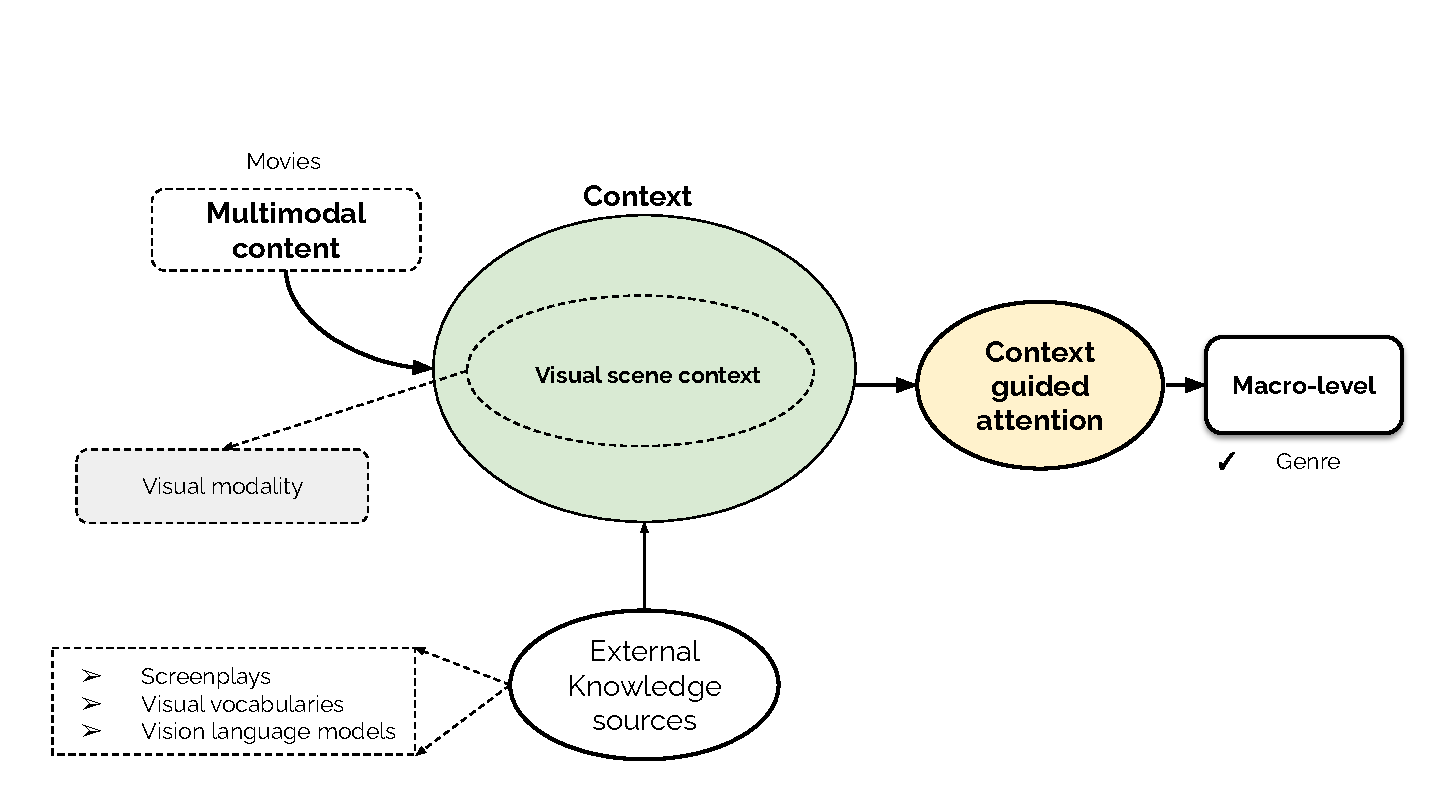
\includegraphics[width=\linewidth]{figures/visual_scene_context.pdf}
     \caption{Overview of visual scene context guided content understanding.}
     \label{visual_scene_context}
\end{figure}


\section{Role of scene as contextual signal}
\begin{figure}[h!]
    \centering 
     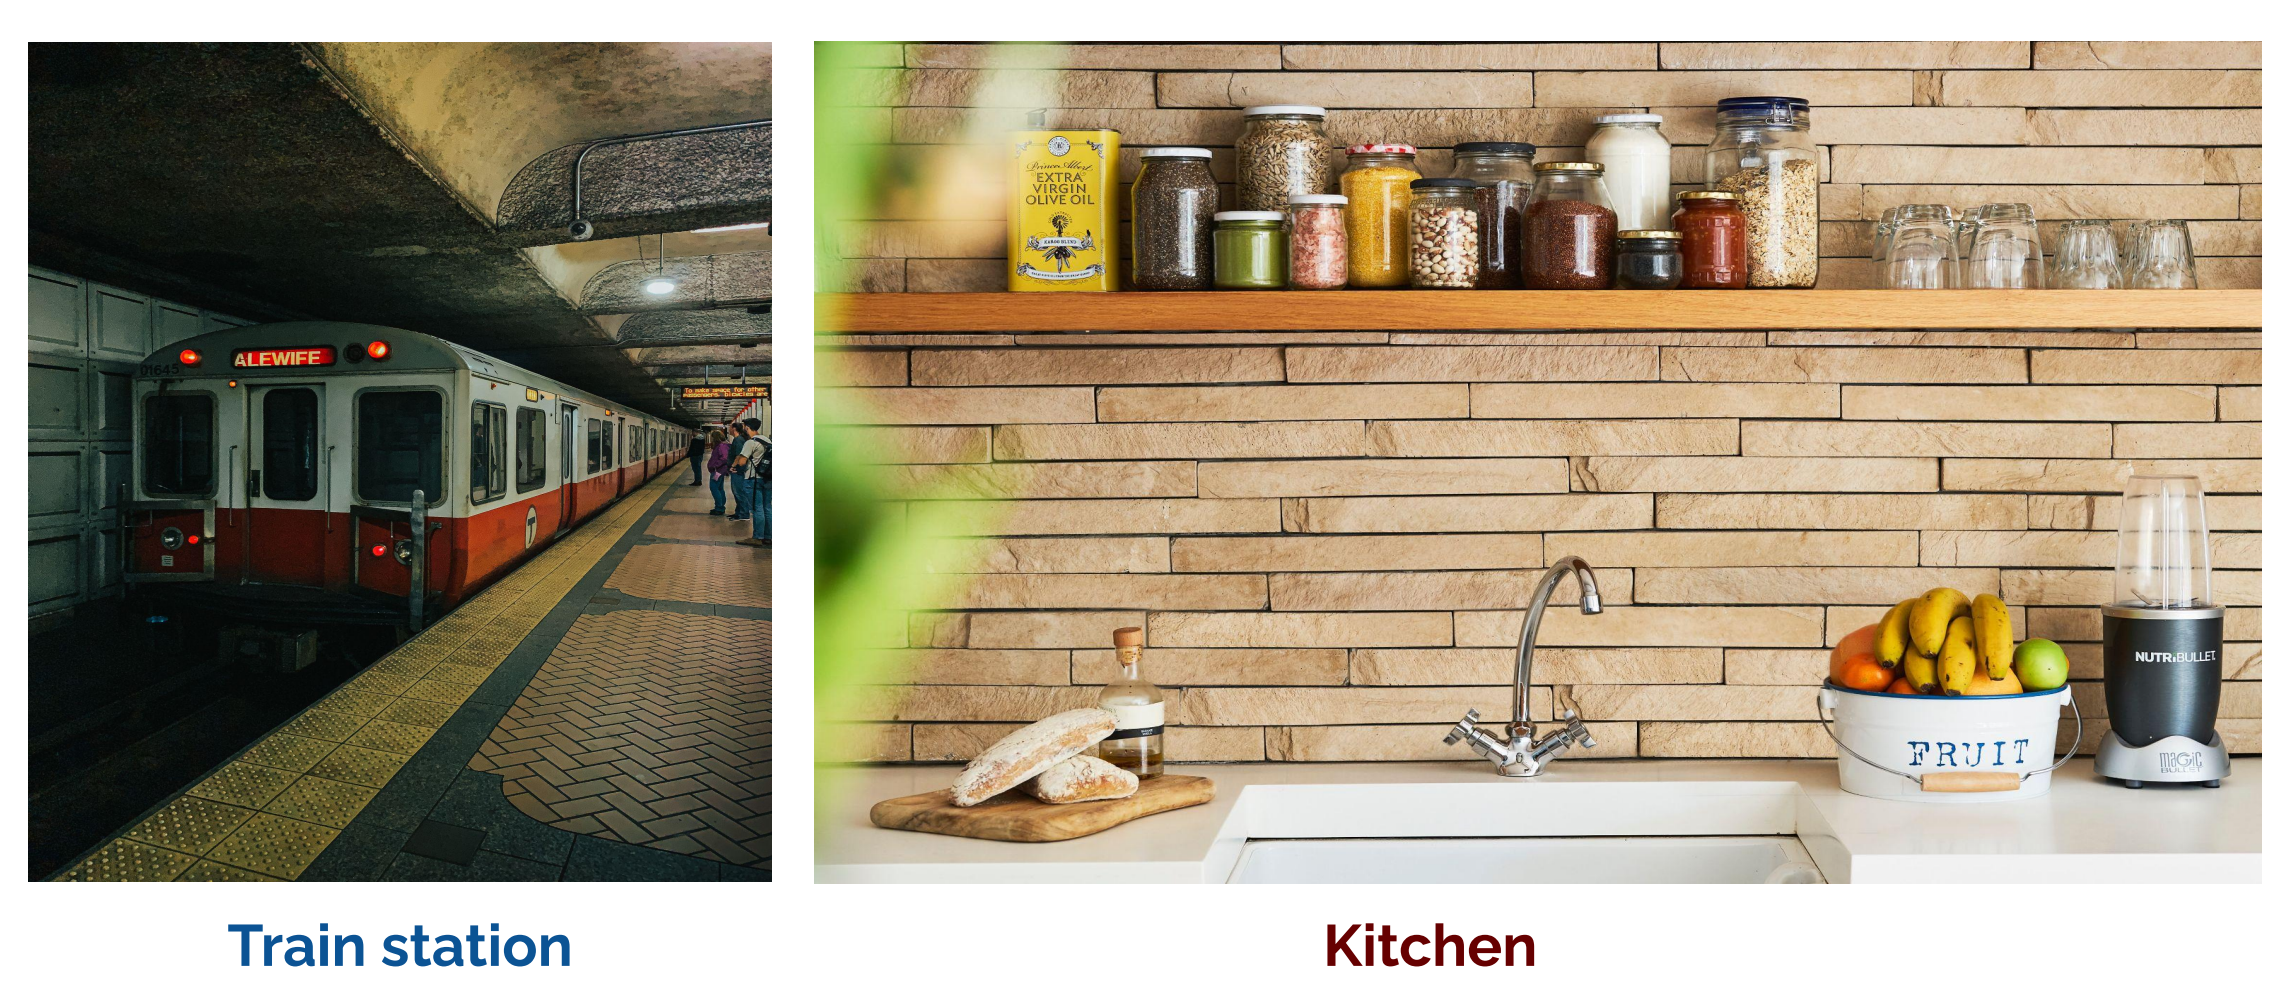
\includegraphics[width=0.6\linewidth]{figures/train_station_kitchen.png}
     \caption{Difference between visual scenes - train station and kitchen in terms of object placements.}
     \label{station_kitchen}
\end{figure}
Visual scene context refers to the global context in the image, including the relationship of the target objects with the environment/location and other co-occurring objects \cite{Bar2004VisualOI}, \cite{Qiao2021ObjectLevelSC}. Visual scene context drives the likelihood of finding particular objects spatially co-located with each other. For example, as shown in Fig \ref{station_kitchen}, utensils are more likely to be present in the kitchen as compared to the train station. 
Apart from the domain of natural scenes, understanding the visual scene context is also important in the case of media content \cite{CMI} esp. movies and curated short content like advertisements. 
\par
In cinematic terms, \textit{mis-en-scene} \cite{Bordwell1979FilmAA} refers to how the different elements of a film are depicted and arranged in front of camera. Key components of \textit{mis-en-scene} include the actors with their different styles, \textbf{visual scenes} where the interactions take place, set design including lighting and camera placement, and the accompanying costumes and makeup of the artists. The visual scene is considered a crucial component since it sets the mood and provides a background for the various actions performed by the actors in the scene. Visual scenes in movies are often tied to social settings like weddings, birthday parties, and workplace gatherings that provide information about character interactions. Accurate recognition of visual scenes can help uncover the bias involved in the portrayal of under-represented characters vis-a-vis different scenes, e.g., fewer women shown in the office as compared to the kitchen. For content tagging tasks like genre classification, visual scenes provide context information like battlefield portrayals in action/adventure movies, space-shuttle in sci-fi movies, or courtrooms in dramas.
In the following section, we highlight certain challenges associated with visual scene recognition, especially w.r.t. movies.
\section{Movies vs Natural scenes}
Visual scene recognition, in the case of static images, is primarily driven by natural scenes due to large-scale datasets like SUN397 \cite{Xiao2010SUNDL} and Places-2\cite{zhou2017places}. However, there are certain inherent challenges in visual scene recognition for movies that need to be addressed, as shown in Fig \ref{Intro figure}.
\begin{figure}[!h]
 \centering
  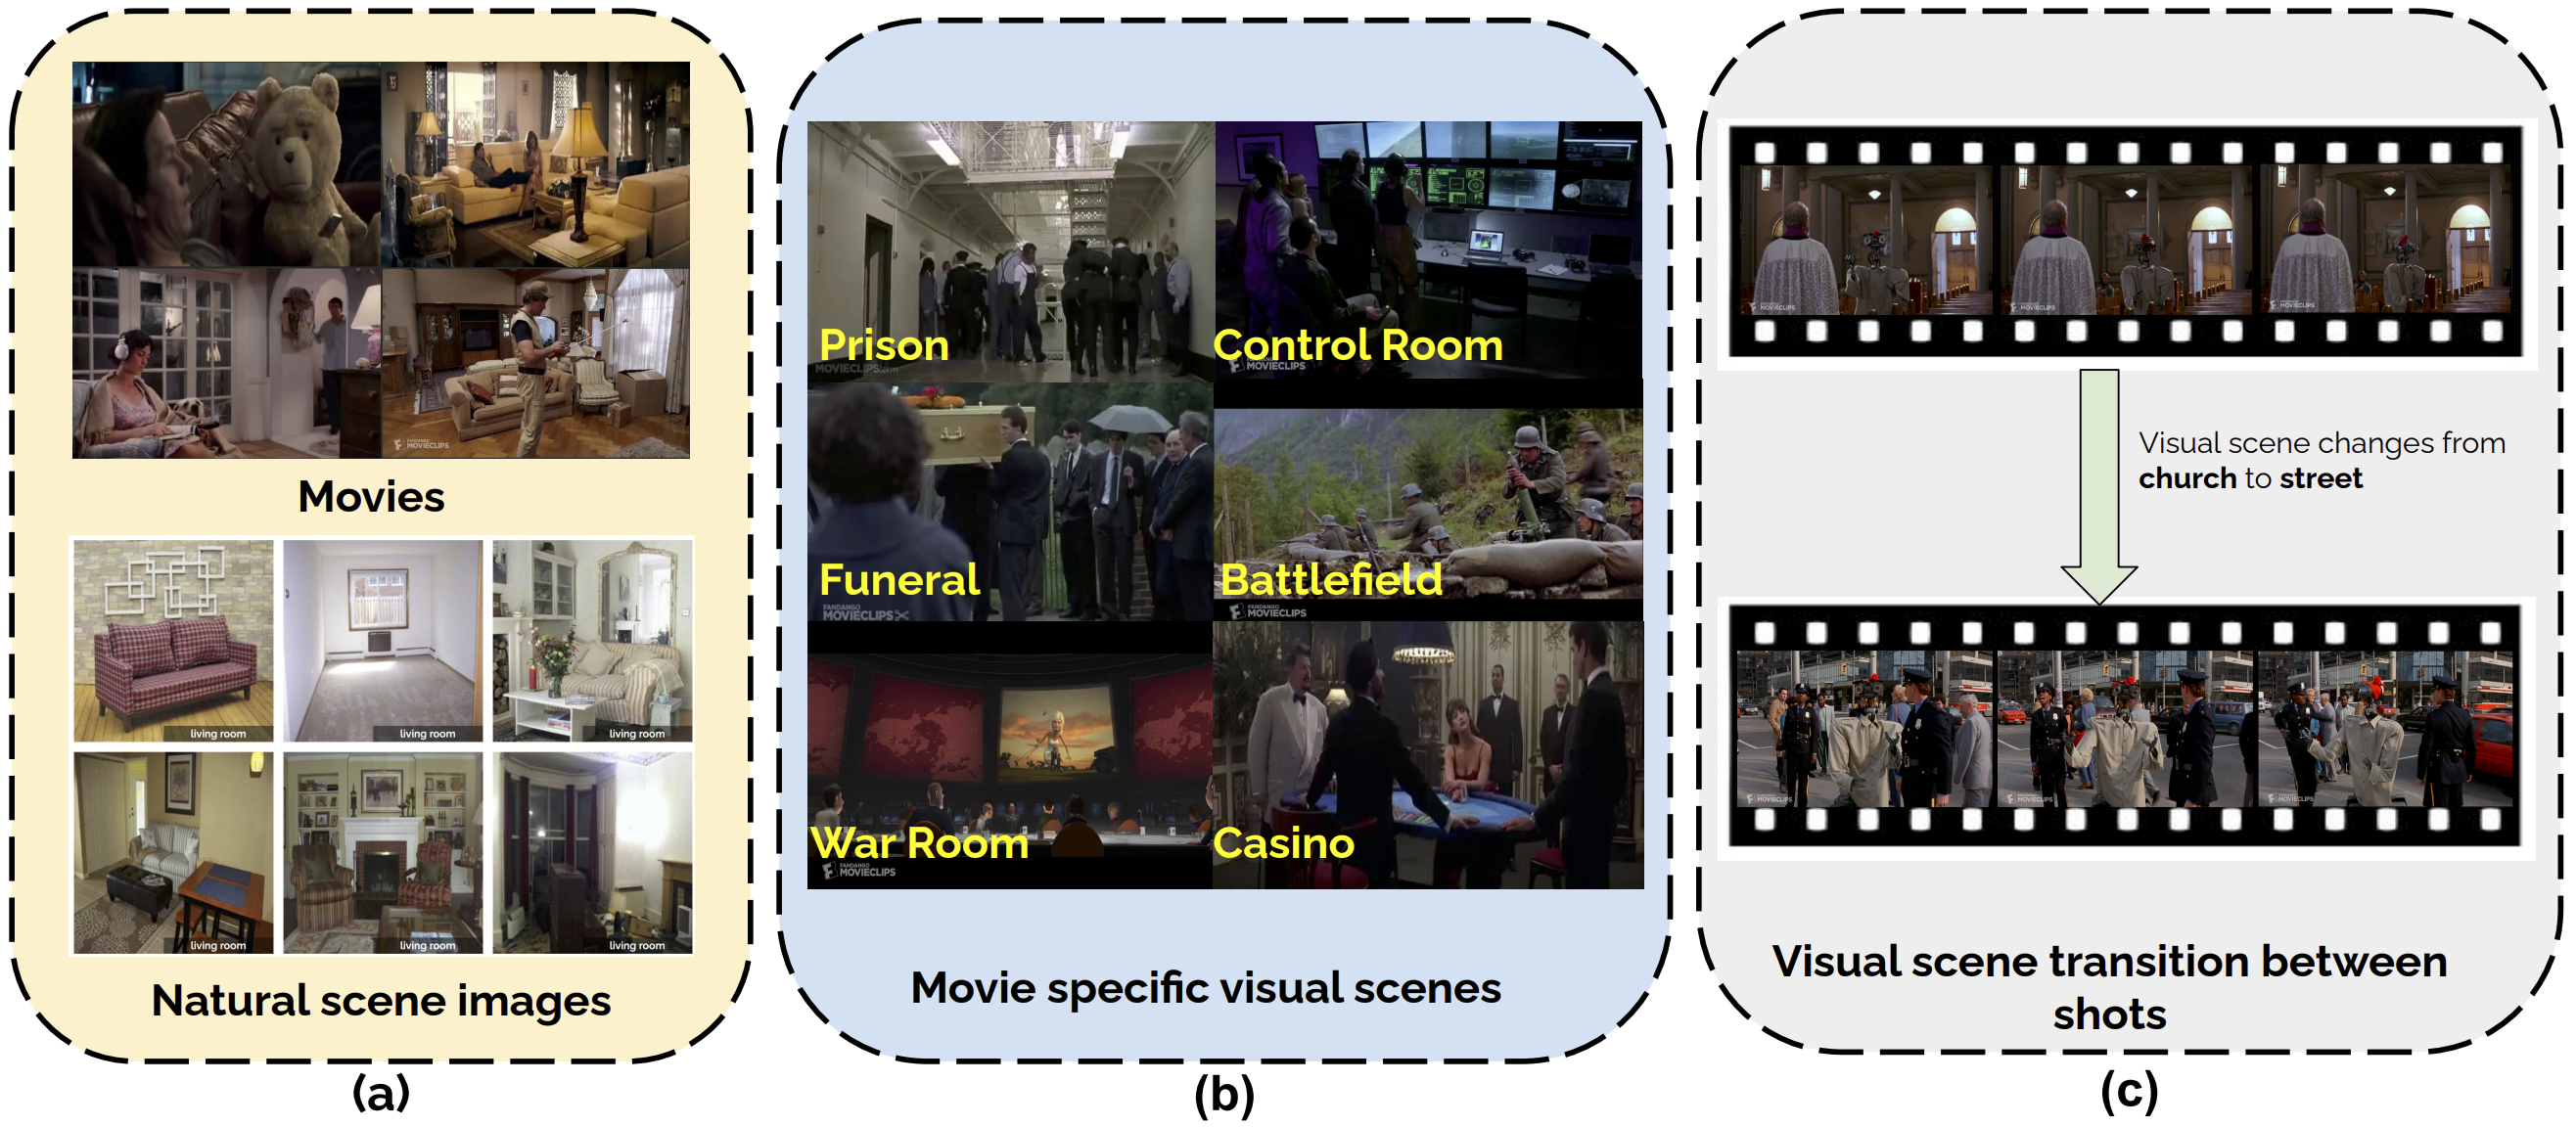
\includegraphics[width=0.8\linewidth]{figures/Introduction_Figure.png}
  \caption{Overview diagram highlighting the challenges associated with visual scene recognition in movies (a) Domain mismatch between Natural scene images,(Source: \url{http://places2.csail.mit.edu/explore.html}) vs frames from Movies for \textbf{living room} (b) Movie centric visual scene classes like prison, control room etc that are absent from existing taxonomies (c) Change in visual scene between shots in the same movie clip.}
  \label{Intro figure}
\end{figure}
\textbf{\underline{Domain mismatch - scene images vs. movie frames:}} Visual scenes depicted in movies are distinct compared to natural scenes due to increased focus on actors, multiple activities, and viewpoint variations like extreme closeup, wide-angle shots etc. An example is shown in Fig.~\ref{Intro figure} (a) for images from Places2 dataset \cite{zhou2017places} and movie frames from Condensed Movies dataset \cite{bain2020condensed}.\\
\textbf{\underline{Lack of completeness in scene taxonomy:}} Movies depict both real-life and fictional scenarios that span a wide variety of visual scenes. As shown in Fig.~\ref{Intro figure}(b), certain movie-centric visual scene classes like \textit{battlefield}, \textit{control room}, \textit{prison}, \textit{war room}, \textit{funeral}, \textit{casino} are absent from existing public scene taxonomies associated with natural scene image and video datasets.\\
\textbf{\underline{Lack of shot-specific visual scene annotations:}} Existing datasets like Condensed Movies \cite{bain2020condensed} and VidSitu \cite{Sadhu_2021_CVPR} provide a {\em single} visual scene label for the entire movie clip (around 2 minutes long), obtained through descriptions provided as part of YouTube channel Fandango Movie clips \footnote{https://www.youtube.com/channel/UC3gNmTGu-TTbFPpfSs5kNkg}. In Fig.~\ref{Intro figure} (c), the provided description: \textit{Johnny Five (Tim Blaney) searches for his humanity in the \textbf{streets} of New York.} mentions only the visual scene \textbf{street}, while the initial set of events takes place inside \textbf{church}. Instead of considering a single scene label for the entire movie clip, shot-level visual scene annotation can help in tracking the scene change from \textbf{church} to \textbf{street}.
\section{Contributions}
In our work, we consider shots within a given movie clip as the fundamental units for visual scene analysis since shots consist of consecutive set of frames related to the same content, whose starting and ending points are triggered by recording using a single camera \cite{SBD}. Our contributions are as follows:
Our contributions are as follows:
\begin{itemize}
\item \textbf{Language guided Movie-centric scene taxonomy:} We develop a movie-centric scene taxonomy by leveraging scene headers (sluglines) from movie scripts (language-based sources) and existing video datasets with scene labels like HVU\cite{diba_large_2020}. 
\item \textbf{Automatic shot tagging:} We utilize our generated scene taxonomy to automatically tag around 1.12M shots from 32K movie clips using a pretrained vision-language model called CLIP \cite{CLIP} based on a frame-wise aggregation scheme.  
\item \textbf{Multi-label scene classification:} We develop multi-label scene classification baselines using the shot-level tagged dataset called MovieCLIP and evaluate them on an independent shot-level dataset curated by human experts. 
\item \textbf{Downstream tasks:} We further extract feature representations from the baseline models pretrained on MovieCLIP and explore their applicability in diverse downstream tasks of multi-label scene and movie genre classification from web videos \cite{diba_large_2020} and trailers \cite{2019Moviescope}, respectively. 
\end{itemize}
\section{Related work}
\textbf{Image datasets for visual scene recognition:}
Image datasets for scene classification like MIT Indoor67 \cite{IndoorScenes} relied on categorizing a finite set of (67) indoor scene classes. A broad categorization into indoor, outdoor (natural) and outdoor (man-made) groups for 130K images across 397 subcategories was introduced by the SUN dataset \cite{xiao_sun_2016}. For large-scale scene recognition, the Places dataset \cite{zhou2017places} was developed with 434 scene labels spanning 10 million images. The scene taxonomy considered in the Places dataset was derived from the SUN dataset, followed by the careful merging of similar pairs. It should be noted that the curation of large-scale visual scene datasets like Places relied on crowd-sourced manual annotations over multiple rounds.\\
\textbf{Video datasets for visual scene recognition:} While there has been considerable progress in terms of action recognition capabilities from videos due to the introduction of large-scale datasets like Kinetics \cite{kinetics400}, ActivityNet \cite{caba2015activitynet}, AVA \cite{gu2018ava}, Something-Something \cite{Something-SomethingV2}, only few large scale datasets like HVU \cite{diba_large_2020} and Scenes, Objects and Actions (SOA) \cite{SOA} have focused on scene categorization with actions and associated objects. SOA was introduced as a multi-task multi-label dataset of social-media videos across 49 scenes with objects and actions but the taxonomy curation involves free-form tagging by human annotators followed by automatic cleanup. 
HVU \cite{diba_large_2020}, a recently released public dataset of web videos with 248 scene labels, relied on initial tag generation based on cloud APIs followed by human verification.\\
\textbf{Movie-centric visual scene recognition:} In the domain of scene recognition from movies, Hollywood scenes \cite{marszalek09} was first introduced with 10 scene classes extracted from headers in movie scripts across 3669 movie clips. A socially grounded approach was explored in Moviegraphs \cite{moviegraphs} with emphasis on the underlying interactions (relationships/situations) along with spatio-temporal localizations and associated visual scenes (59 classes).
For holistic movie understanding tasks, the Movienet dataset\cite{huang2020movienet} was introduced with the largest movie-centric scene taxonomy consisting of 90 place (visual scene) tags with segment-wise human annotations of entire movies. Instead of entire movie data, short movie clips sourced from YouTube channel of Fandango Movie clips were used for text-video retrieval in Condensed movies dataset \cite{bain2020condensed}, visual semantic role labeling \cite{Sadhu_2021_CVPR} and pretraining object-centric transformers \cite{transformers} for long-term video understanding in LVU dataset \cite{lvu2021}. While there is no explicit visual scene labeling, the raw descriptions available on Youtube with the movie clips have mentions of certain visual scene classes.
\\
MovieCLIP, our curated dataset for visual scene context recognition, is built on top of movie clips available as a part of Condensed Movies dataset \cite{bain2020condensed}. A comparative overview of MovieCLIP and other image and video datasets with visual scene labels is shown in Table~\ref{Overview}. In comparison with previous video-centric works, our taxonomy generation relies on domain-centric data sources like movie scripts and auxiliary world knowledge from web-video-based sources like HVU with minimal human-in-the-loop supervision for taxonomy refinement.
\begin{table*}[h!]
\centering
\resizebox{0.8\textwidth}{!}{
\begin{tabular}{|c|c|c|c|c|c|c|}
\hline
\textbf{Dataset} & \textbf{Domain} & \textbf{\#classes} & \textbf{\#samples} & \textbf{Annotation} & \textbf{Unit} & \textbf{AV} \\ \hline
Scene 15 \cite{BayesianFeiFeiLi}   & Natural & 15  & $\sim$6k   & Manual & Image  & \cmark     \\ \hline
MITIndoor67  \cite{IndoorScenes} & Natural     & 67   & 15620   & Manual  & Image &\cmark    \\ \hline
SUN397  \cite{xiao_sun_2016}   & Natural    & 397   & 130,519  & Manual  & Image &\cmark    \\ \hline
Places  \cite{zhou2017places}    & Natural   & 434   & 10m  & Manual  & Image & \cmark     \\ \hline
Hollywood Scenes \cite{marszalek09}   &  Movies    & 10    & 3669   & Automatic  & Video clip (36.1s)  & \cmark  \\ \hline
Moviegraphs  \cite{moviegraphs}    & Movies   & 59     & 7637   & Manual  & Video clip (44.28 s)  & \xmark    \\ \hline
SOA \cite{SOA} &  Web-Videos   & 49   & 562K   & Semi-automatic  & Video clip (10 s)  &   \xmark      \\ \hline
Movienet  \cite{huang2020movienet}  & Movies   & 90    & 42K  & Manual  & Scene segment (2 min)  & \xmark           \\ \hline
HVU    \cite{diba_large_2020}    & Web-Videos    & 248    & 251k  & Semi-automatic &  Video clip (10 s) & \cmark    \\ \hline
Condensed Movies \cite{bain2020condensed}   & Movies    & NA    & 33k   & Automatic  & Video clip ( 2 min) & \cmark    \\ \hline
VidSitu  \cite{Sadhu_2021_CVPR}    & Movies  & $\sim$50    & 14k   & Manual  & Video  clip (10 s) & \cmark     \\ \hline
LVU  \cite{lvu2021}    & Movies    & 6    & 723   & Automatic &  Video clip ($1 \sim 3$ min) & \cmark       \\ \hline
\textbf{MovieCLIP}  & \textbf{Movies}  & \textbf{179}  & \textbf{1.12m}& \textbf{Automatic} & \textbf{Shot (3.54s) }  & \textbf{\cmark }    \\ \hline
\end{tabular}
}
\vspace{5mm}
\caption{Comparison of MovieCLIP with other available image and video datasets with visual scene classes.  \textbf{Natural}: Images of natural scenes.\textbf{Web-Videos}: videos obtained from internet sources like YouTube. \textbf{AV}: whether publicly available or not. Avg or duration span of video data sources are provided with the respective units. \textbf{NA}: Number of scene classes explicitly not mentioned with the dataset.}
\label{Overview}
\end{table*}
\\
\textbf{Knowledge transfer from pretrained multimodal models:}
Vision language(V-L) based pretraining methods involve learning transferable visual representations based on various pretext tasks associated with image and text pairs. Examples of pretext tasks in V-L domain include prediction of masked words in captions based on visual cues in ICMLM \cite{sariyildiz2020icmlm}, pretraining image encoders based on bicaptioning objective in VirTex \cite{desai2021virtex} and contrastive alignment of image-caption pairs in CLIP \cite{CLIP}. Leveraging features from CLIP's visual and text encoders have improved existing vision-language tasks \cite{Shen2021HowMC} and enabled open-vocabulary object detection \cite{Gu2021OpenvocabularyOD}, and language-driven semantic segmentation \cite{Li2022LanguagedrivenSS}. In our work, we use the pretrained visual and text encoders of CLIP and utilize it as a noisy annotator by tagging movie shots based on our curated visual scene taxonomy.

\section{Language driven taxonomy curation}

Based on domain-specific challenges mentioned in Fig \ref{Intro figure}, we can see the need for a taxonomy curation phase for visual scenes in movies. In this section, we outline the process involved in curating a visual scene taxonomy based on the domain information present in movie scripts and the pre-existing scene information present in auxiliary video datasets.

\subsection{Sources of visual scene information}
Movie scripts have been used as external sources for describing and annotating videos through script and subtitle alignment methods in \cite{10.1007/978-3-540-88693-8_12}, \cite{Everingham2006HelloMN}, \cite{Laptevactionscvpr}, \cite{Rohrbach2015ADF}. Movie scripts contain \textit{sluglines} that provide information about visual scenes, time of the day, and whether the action takes place in indoor or outdoor settings.

\begin{figure}[!h]
 \centering
  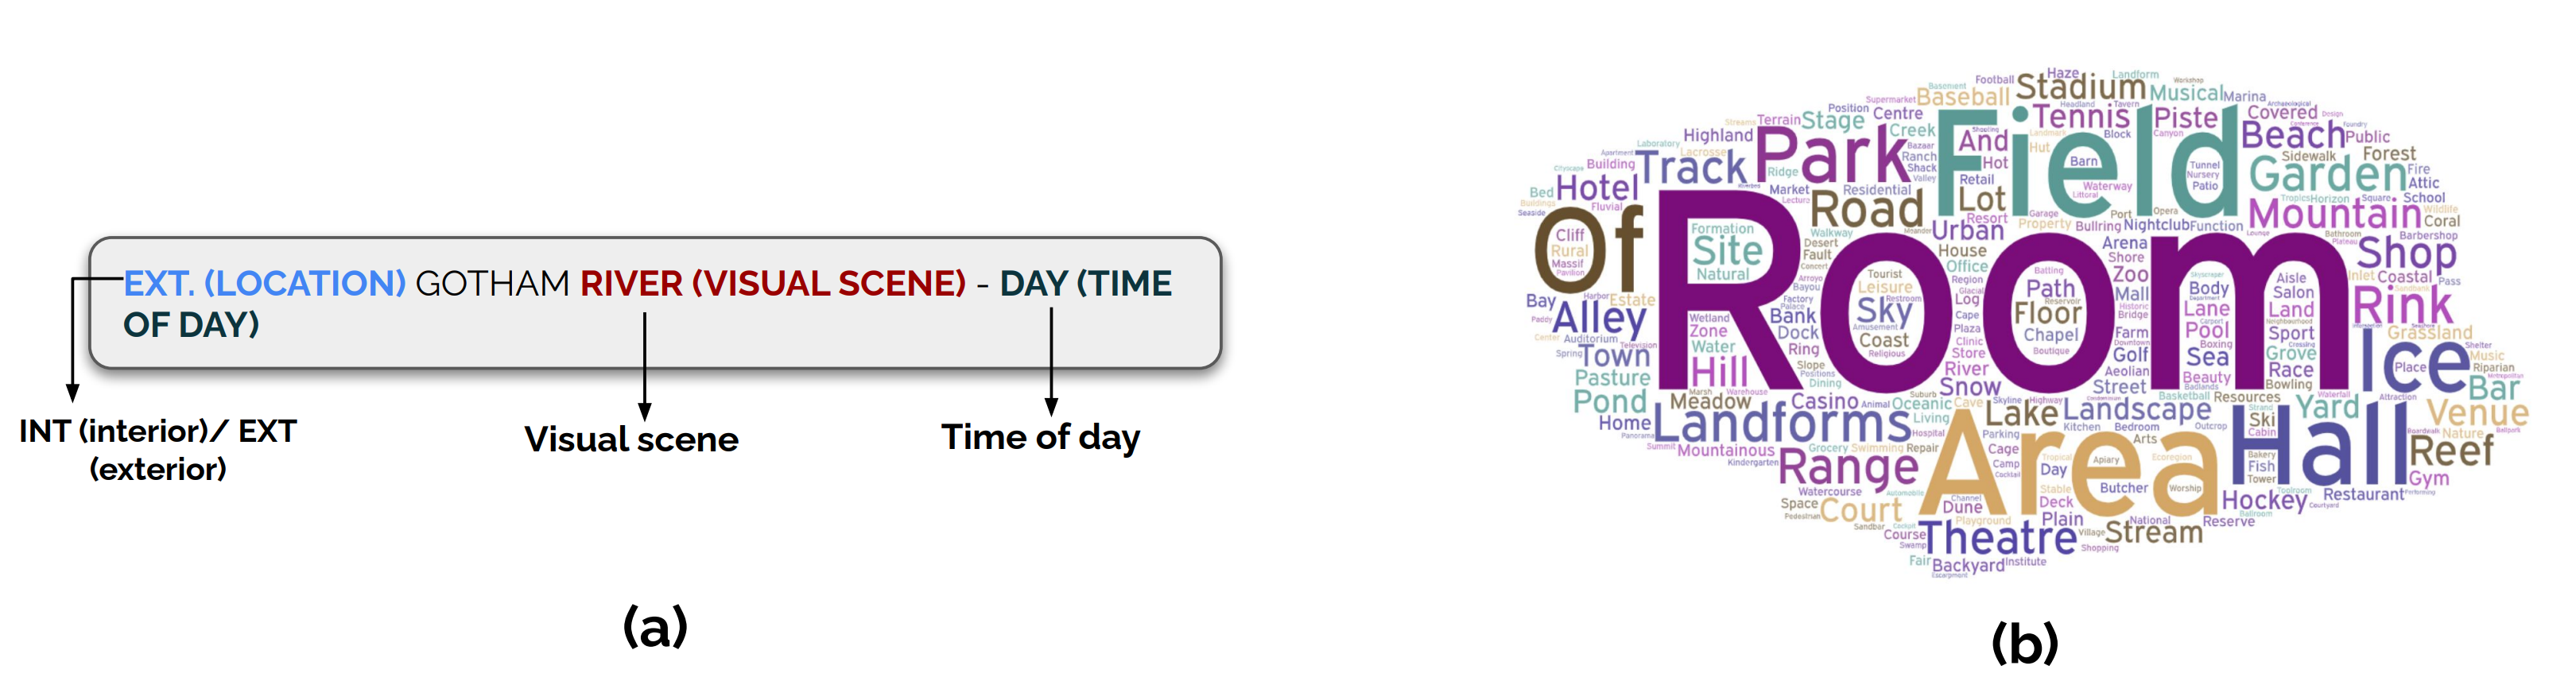
\includegraphics[width=\linewidth]{figures/sources_of_information_visual_scene_taxonomy.png}
  \caption{Sources of visual scene information: (a) Sample slugline from a movie script that contains visual scene, time of day, and location (b) Word cloud showing the distribution of visual scene labels in HVU \cite{diba_large_2020} dataset.}
  \label{sources of information}
\end{figure}

We parse 156k sluglines from an in-house set of 1434 movie scripts. For each slugline, we automatically extract entities after the ``\textbf{EXT.}''(exterior) or ``\textbf{INT.}''(interior) tags like \textit{Hospital room}, \textit{River}, \textit{War room} etc.
Using this procedure, we extract 173 unique visual scene labels. Our taxonomy generation process is motivated by visual scenes in movies with sluglines from scripts as seed sources along with auxiliary sources.
Since the set of labels from movie scripts is not exhaustive, we also consider auxiliary sources, especially web video datasets with visual scene labels like HVU \cite{diba_large_2020}. We consider HVU as source of additional labels since the taxonomy (248 visual scene classes) is semi-automatically curated for short-trimmed videos, having similar nature to movie shots. We don’t consider Places2 \cite{zhou2017places} dataset since the taxonomy is primarily curated for natural
scenes, which are distinct from movie-centric visual scenes. Sample slugline from a movie script and a word cloud showing the distribution of visual scene labels is shown in Fig \ref{sources of information}.

\subsection{Visual scene taxonomy curation}
In order to develop a comprehensive taxonomy of visual scenes in movies, we develop an automatic way of merging taxonomies from movie sluglines and the auxiliary dataset i.e., HVU with minimal human-in-the-loop for post-processing. The broad steps involved in the taxonomy generation are listed as below:
\par
\textbf{Label space preprocessing:} For simplicity, we consider the set of unique labels from movie sluglines (MS) to be denoted as $L_{MS}$ and its cardinality as $N_{MS}$. Similarly we denote $N_{HVU}$ to be the cardinality of the set $L_{HVU}$, i.e., the set of unique labels from the HVU dataset. For our case, we have $N_{MS}=173$ and $N_{HVU}=248$. We extract the intersecting set of labels between $L_{MS}$ and $L_{HVU}$, denoted by the set $L_{com}$ . The number of common labels between HVU and movie slugline based taxonomy is $N_{com}=68$. We remove the common set of labels $L_{com}$ from both the label spaces of movie sluglines and HVU. This gives us a non-intersecting set of labels in movie sluglines and HVU denoted by $L_{MS} \setminus L_{Com}$  and $L_{HVU} \setminus L_{Com}$ respectively.  We combine the sets of labels i.e. $L_{MS} \setminus L_{Com}$ and $L_{HVU} \setminus L_{Com}$ to obtain a larger set of labels called $L_{NC}$, where NC refers to not common. 
\begin{equation}
    L_{NC}=(L_{MS} \setminus L_{Com}) \cup (L_{HVU} \setminus L_{Com})
\end{equation}
\par 
\textbf{Merging with common label space:}
In this step, we find labels in $L_{NC}$ that are semantically close to the labels in $L_{com}$. We extract dense 384D label representations using the MiniLM-L6-v2 sentence transformers model \cite{reimers-2019-sentence-bert} for labels in $L_{NC}$ and $L_{com}$. For each label in $L_{NC}$ we compute cosine similarities with set of labels in $L_{com}$ based on label representations. We merge those labels from $L_{NC}$ with the similar labels in $L_{com}$, whose top-1 cosine similarity values are greater than 0.6. We update the set of labels $L_{NC}$ to $L_{N}$ by removing the merged labels.
Examples of such merging with respective cosine similarities and sources are as follows:
\begin{itemize}
    \item $\textbf{dune} \{L_{NC}\} \rightarrow{} \textbf{desert} \{L_{com}\} (0.66)$ 
    \item $\textbf{tennis} \ camp \{L_{NC}\} \rightarrow{} \textbf{tennis \ court} \{L_{com}\}  (0.62)$
    \item $\textbf{restroom} \{L_{NC}\} \rightarrow{} \textbf{bathroom} \{L_{com}\} (0.80)$
    \item $\textbf{rural \ area} \{L_{NC}\} \rightarrow{} \textbf{village} \{L_{com}\} (0.64)$
    \item $\textbf{boardwalk} \{L_{NC}\} \rightarrow{} \textbf{walkway} \{L_{com}\} (0.67)$
    \item $\textbf{television \ room} \{L_{NC}\} \rightarrow{} \textbf{living \ room} \{L_{com}\} (0.67)$
    \item $\textbf{glacial \ lake} \{L_{NC}\} \rightarrow{} \textbf{lake} \{L_{com}\} (0.73)$
\end{itemize}

\begin{figure}[h!]
\centering
%\subfloat[]{%
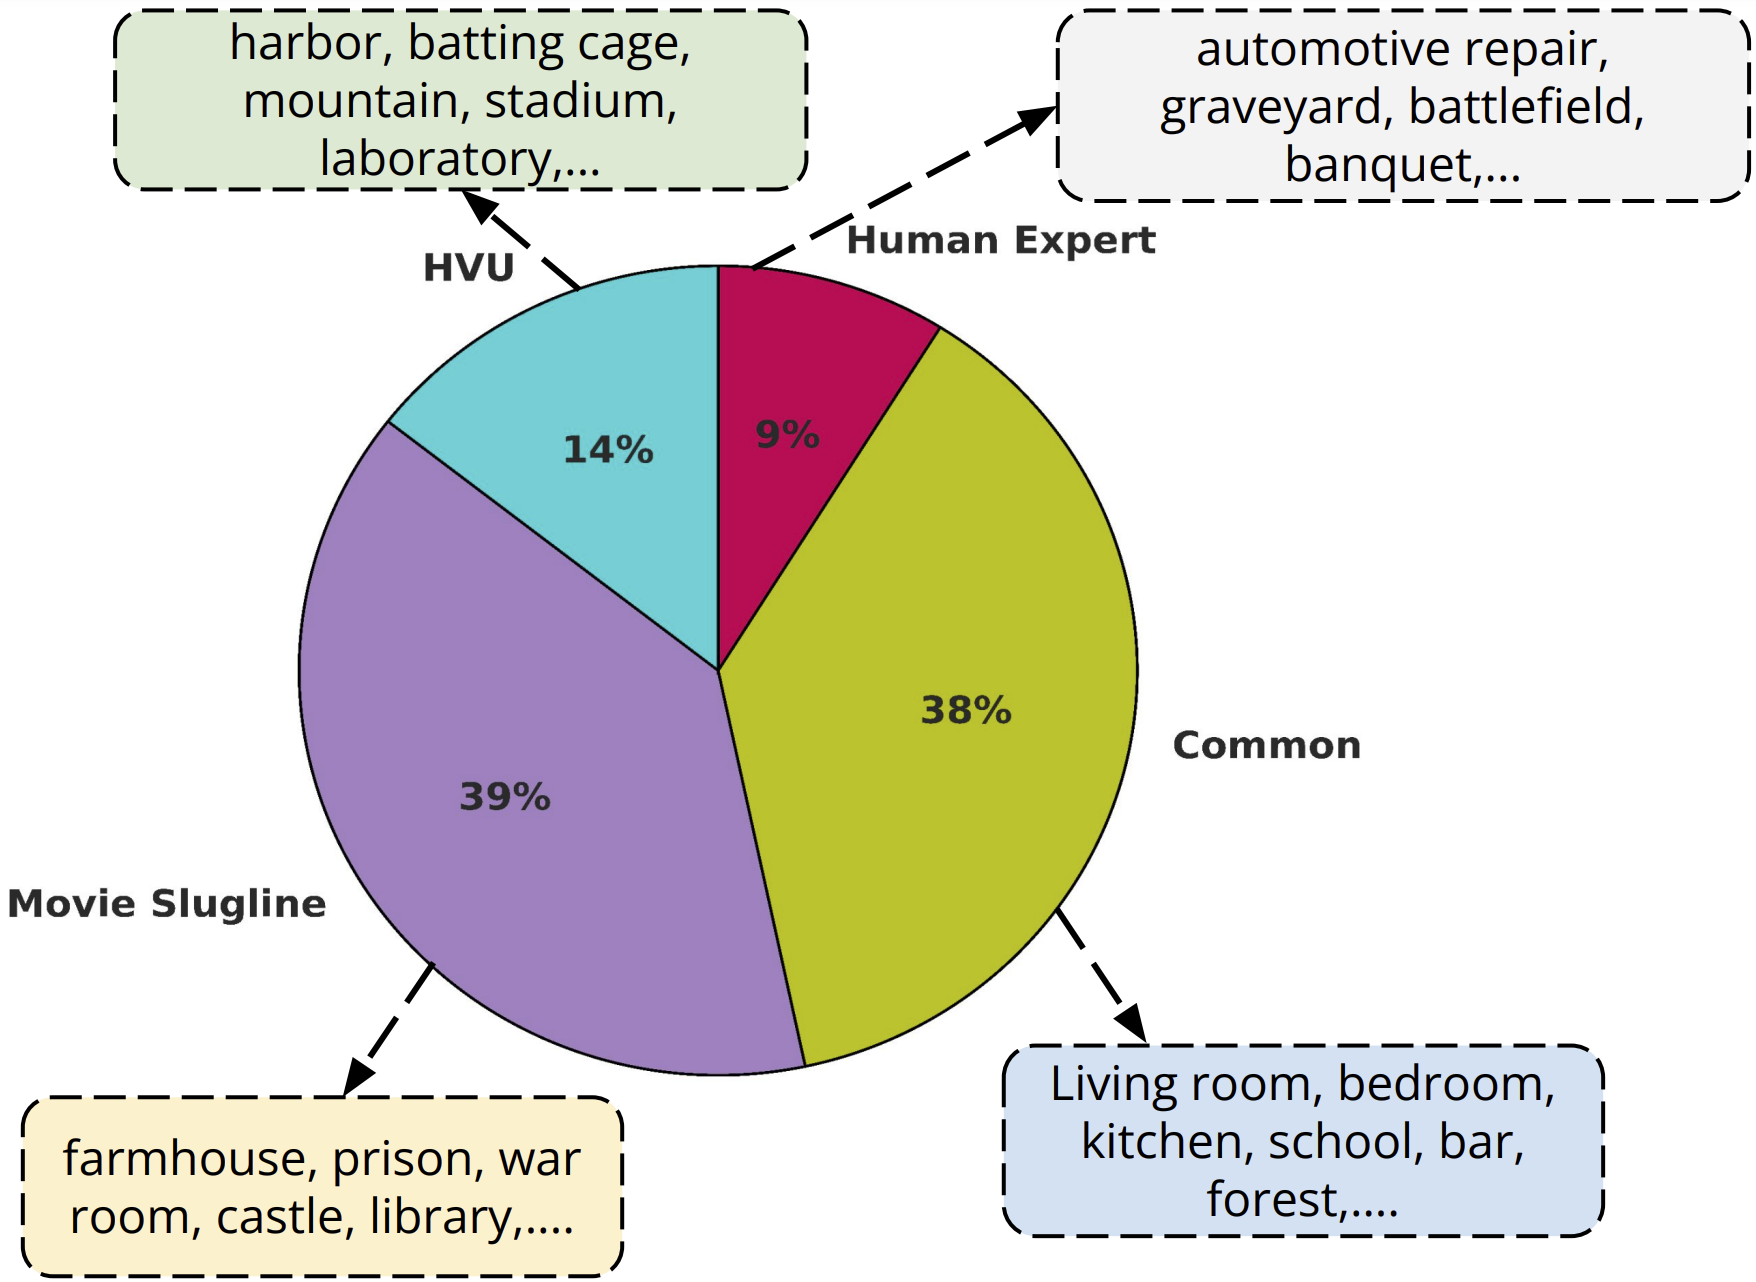
\includegraphics[width=0.6\columnwidth]{figures/share_of_labels.png}%
\caption{
The share of different sources (\textbf{HVU}, \textbf{Movie Sluglines}, \textbf{Common labels and Human expert}) in curating the label taxonomy. Example labels from different sources are shown in boxes with the pie chart.
}
\label{label distribution}
\end{figure}
\textbf{Human-in-the-loop taxonomy refinement:} 
A human expert inspects the labels in $L_{N}$ and removes both generic scene labels such as \textit{body of water}, \textit{coastal and oceanic landforms}, \textit{horizon}, \textit{landscape}, \textit{underground} as well as highly specific scenes such as \textit{coral reef}, \textit{white house}, \textit{piste}, \textit{badlands} etc. We use label representations from the previous step to exploit semantic similarity between the labels remaining in $L_{N}$.
For each relevant label in $L_{N}$, a threshold of 0.7 on top-1 similarity score is used to filter out similar labels. While comparing two similar labels, the human expert relies on wiki definitions to merge the more specific label into the generic one. For example, by definition \textit{bazaar} is a special form of market selling local items (as per wiki) and therefore merged with the \textit{market}. Other examples include:
\begin{itemize}
    \item $\{stream, river bed, creek, river\} \rightarrow{} river$ 
    \item $\{hill, mountain, mountain \ pass, mountain \ range\} \\ \rightarrow{} mountain$
    \item $\{road, road \ highway, lane \} \rightarrow{} road$
    \item $\{port, marina \ dock, harbor \} \rightarrow{} harbor$
\end{itemize}
This results in a set of labels called $L_{merge}$ from $L_{N}$. Further, The human expert is exposed to randomly sampled 1000 shots from movie clips in Condensed Movies \cite{bain2020condensed} and reviews the current set of labels in the set $L_{merge} \cup L_{com}$. Based on the video content, a set of scene labels ($L_{human}$) that are missing from the current set is added by human expert. Thus the final set of 179 visual scene labels is obtained as follows:
\begin{equation}
     L_{final}=L_{com}\cup L_{merge} \cup L_{human}
\end{equation}
\textbf{Label source distribution:} As shown in Fig. \ref{label distribution}, the largest share is from movie sluglines (39\%).Only 9\% of the total labels is provided through feedback from human expert. Instead of manually binning classes into broad categories like indoor, outdoor or man-made, we discover groupings among classes through Affinity propagation clustering \cite{brendanfrey}  (based on label representations from sentence transformers). Certain clusters of visual scene labels are listed below, where all the sport locations, water bodies and performing arts locations are grouped together.
\begin{itemize}
    \item \textbf{sport locations:} Basketball court, Race track, Tennis court, Batting cage, Golf course
    \item \textbf{water bodies:} River, Pool, Waterfall, Hot spring, Pond, Swamp, Lake
    \item \textbf{performing arts locations:} Stage, Conference Room, Theater, Auditorium, Ballroom
    \item \textbf{Natural landforms:} Mountain, Desert, Valley
\end{itemize}
For visualizing certain groups of visual scene classes that are semantically close to each other, we use tSNE \cite{tSNE} to project the 384 D label embeddings obtained through MiniLM-L6-v2 sentence transformers model \cite{reimers-2019-sentence-bert} to 2 dimensions. Examples include the visual scene classes associated with \textbf{study}, \textbf{water bodies} , \textbf{medical scene classes}, \textbf{natural landforms}, \textbf{automobile-based scene classes}, \textbf{dining-scene classes}.
\begin{figure*}[h!]
    \centering
    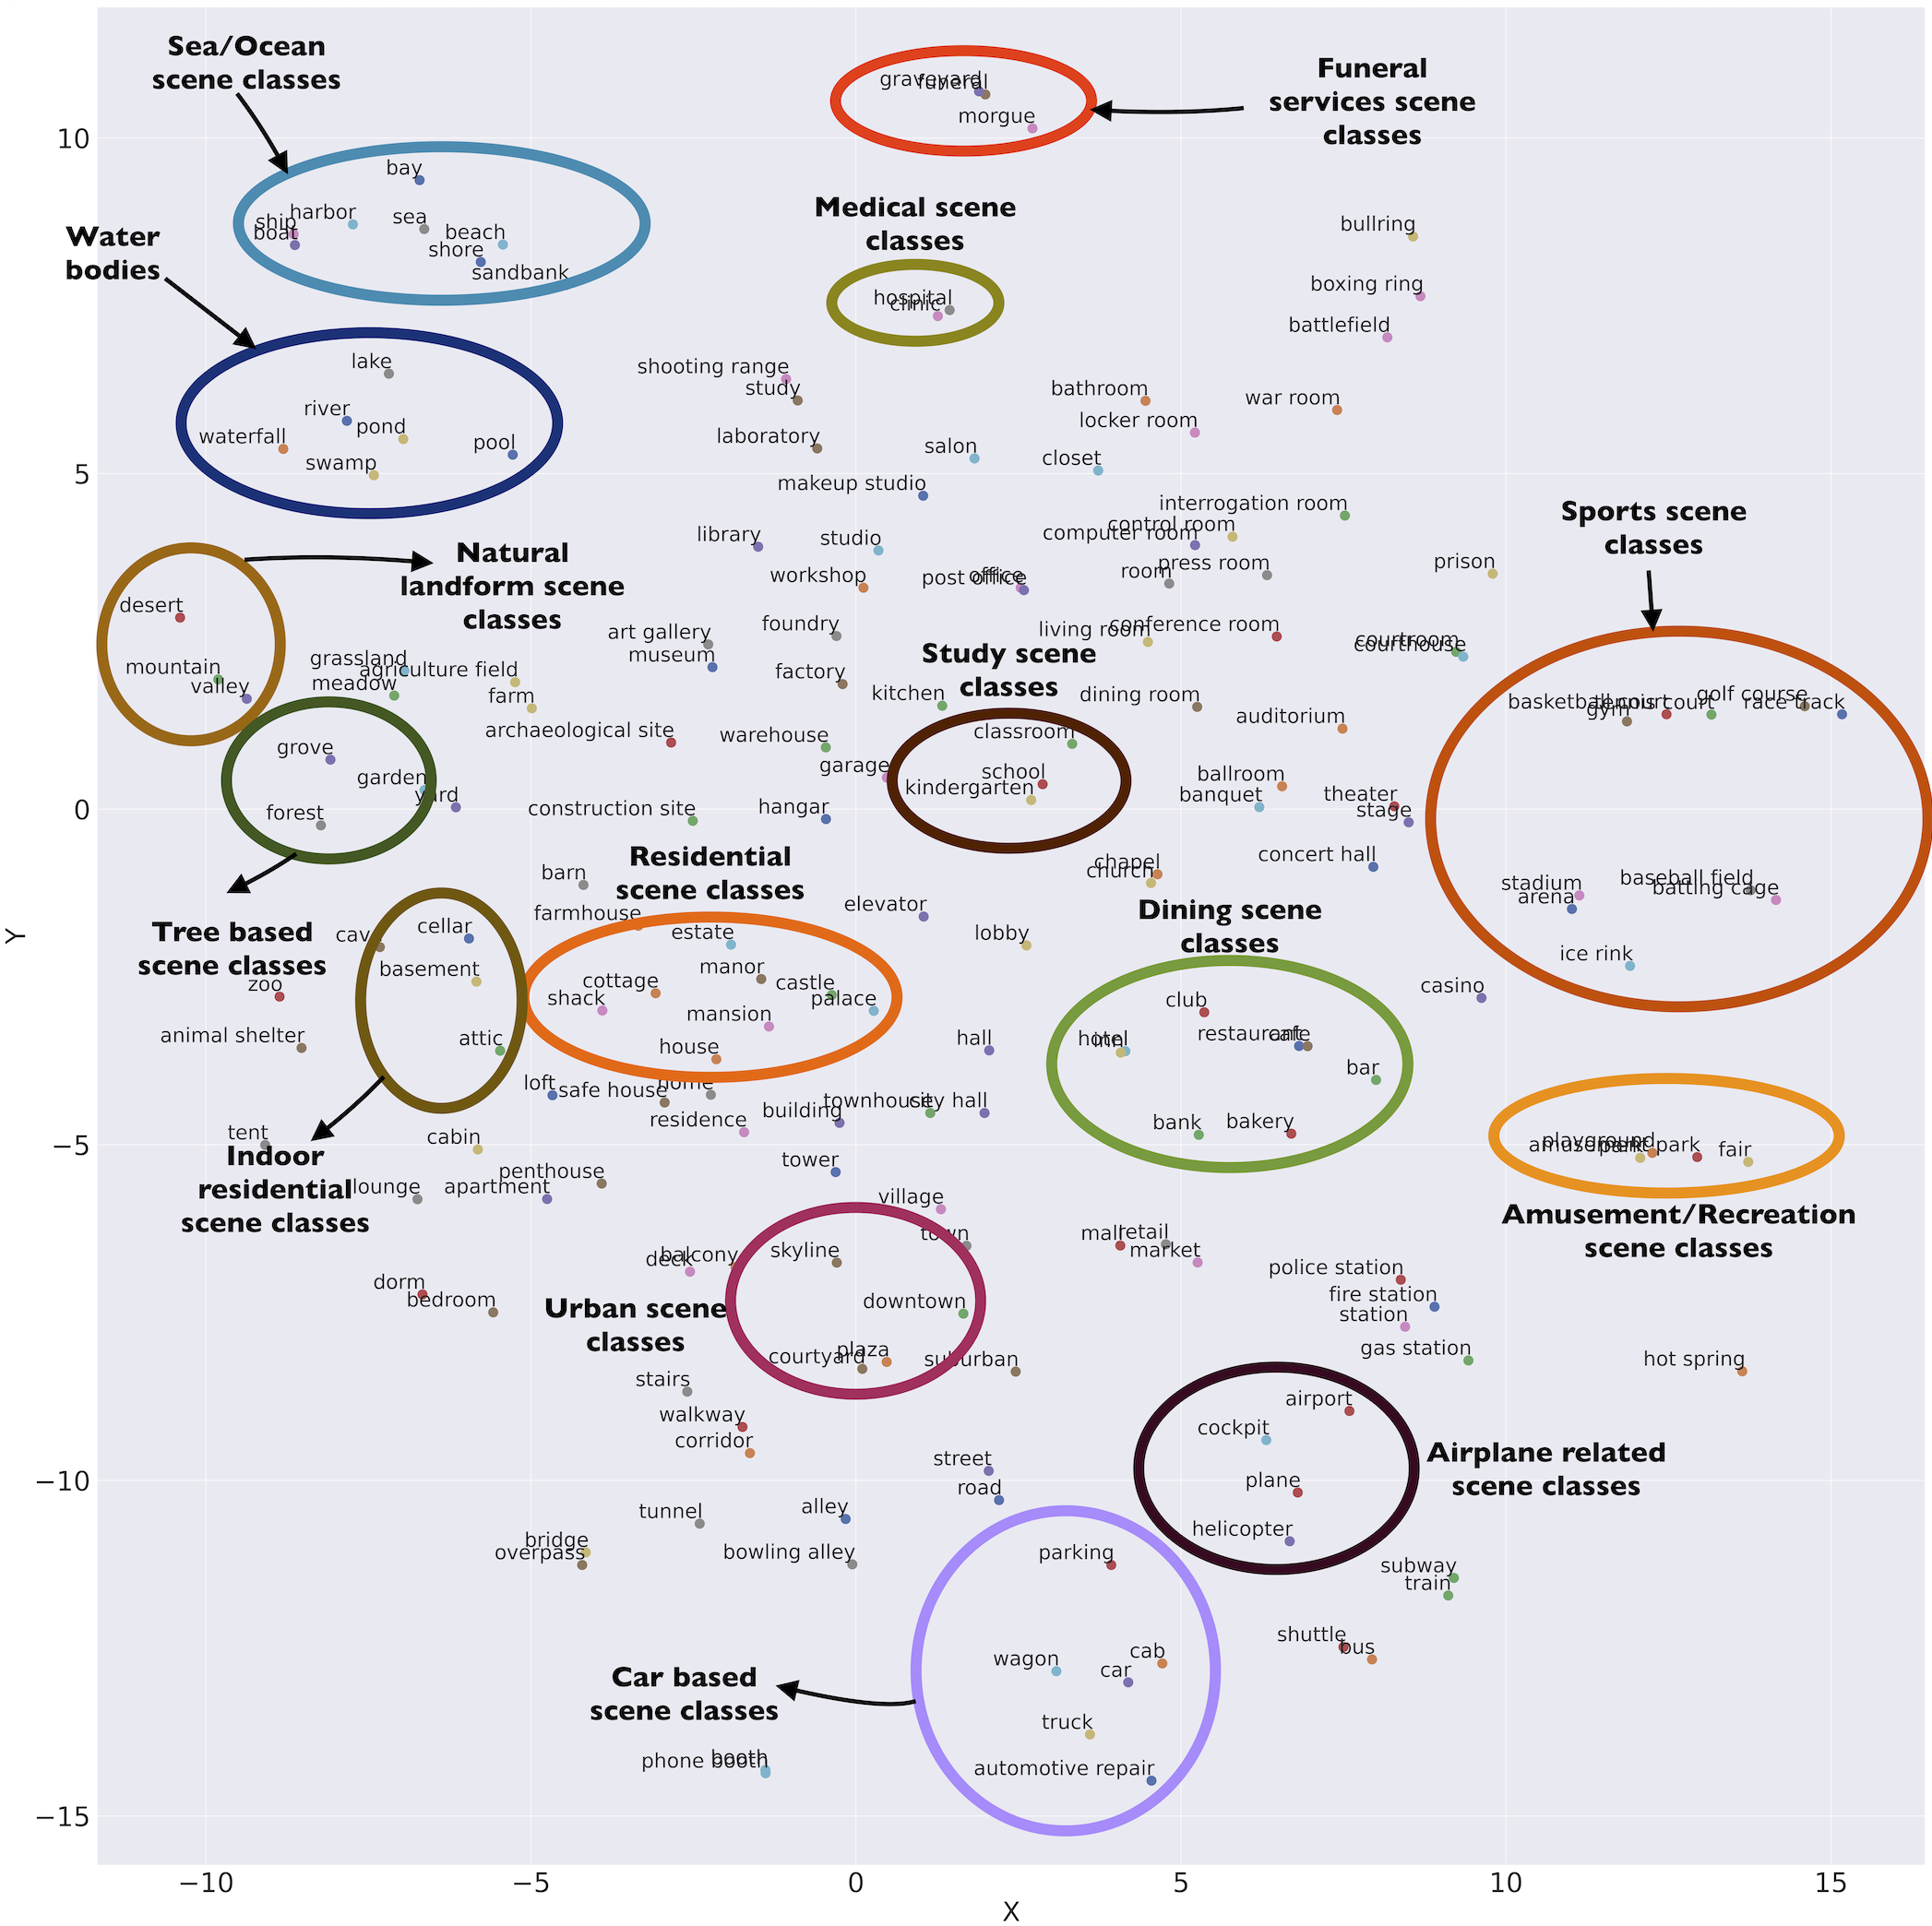
\includegraphics[width=0.9\textwidth]{figures/tsne_hvu_slugline_combined.png}
    \caption{TSNE plot of the 179 scene classes in the taxonomy. Certain representative groups of visual scene labels that are semantically close to each other are enclosed by circular/oval shapes. }
    \label{tsneplot}
\end{figure*}

\section{Role of multi-modality - Usage of vision-language models}

Since the manual tagging of Condensed Movies \cite{bain2020condensed} is not feasible due to the duration of data involved, i.e., \textbf{1106 hrs},  we ask the following question:  \textit{Can we use additional knowledge sources to provide weak guidance for the tagging task ?}. In this case, we leverage the pretrained knowledge available as part of CLIP \cite{CLIP}'s vision and language encoders to provide weak guidance for visual scene labeling. 

\begin{figure}[h!]
\centering
  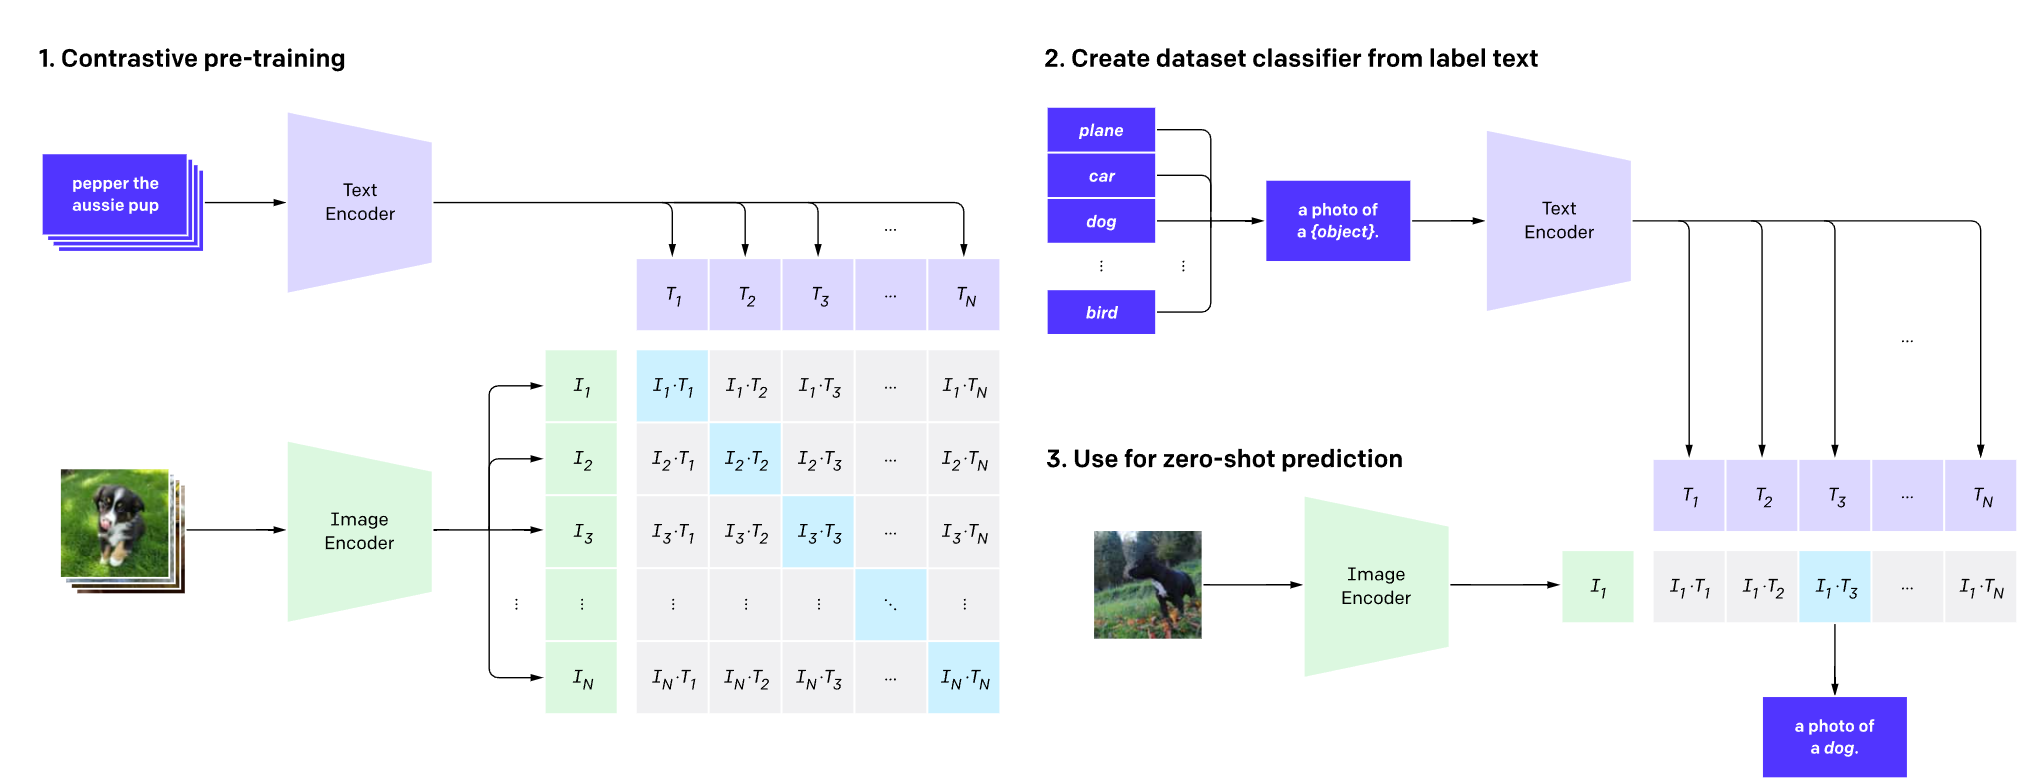
\includegraphics[width=\linewidth]{figures/CLIP_outline_diagram.png}
  \caption{1. Contrastive pretraining framework associated with CLIP. 2. Usage of CLIP's pretrained vision and text encoders for zero-shot classification. Image source: \cite{CLIP}}
  \label{CLIP outline}
\end{figure}
We utilize the pretrained knowledge available in CLIP for weakly tagging the movie video clips with scene labels from our curated taxonomy. 
CLIP utilizes internet-scale data, i.e., image-text pairs, to pre-train two visual and text transformer \cite{transformers} encoders for weak-alignment pretext task. Based on the large batch size of 32,768 image-text pairs, the proxy training task is defined as follows: \textit{given an image, predict which out of a set of 32,768 randomly sampled text snippets, was actually paired with it in our dataset ?}.  Since CLIP has been trained in a contrastive manner for alignment, it can be used to develop zero-shot classifiers for different tasks including scene recognition (\cite{xiao_sun_2016}), fine-grained classification (\cite{parkhi12a}, \cite{bossard14}, \cite{KrauseStarkDengFei-Fei_3DRR2013}), facial emotion recognition (\cite{BarsoumICMI2016}), object (\cite{Deng2009ImageNetAL},\cite{FeiFei2004LearningGV}) and action classification (\cite{Kinetics700},\cite{ucf101}).

In the following section, we outline how CLIP's pretrained encoders are used for tagging shots in the Condensed movies dataset \cite{bain2020condensed} to obtain a curated shot-centric dataset called \textbf{MovieCLIP} with visual scene labels.

\section{MovieCLIP dataset}

\subsection{Shot detection from movie clips}
Since a shot represents a continuous set of frames with minimal change in the visual scene, we consider movie shots for our subsequent analysis. Associating visual scene labels to shots can help in identifying cases where visual scene recognition is difficult like closeup or extreme closeup scenarios, even within the same movie scene. A singular movie scene involves changes in camera viewpoints across consecutive shots, thus making it difficult for CLIP to associate labels with high confidence for the entire movie scene.
For shot detection, we use PySceneDetect\footnote{https://pyscenedetect.readthedocs.io/en/latest/} to segment the movie clips in Condensed Movies with default parameters and content-aware detection mode. The overall statistics of the shot extraction process is shown in Table \ref{shot stats table}:

\begin{table}[h!]
\centering 
\resizebox{\columnwidth}{!}{
\begin{tabular}{|l|c|l|l|l|l|l|}
\hline
\textbf{\# movies} & \textbf{Years} & \textbf{\# clips}    & \textbf{\# shots} & \textbf{Avg shots/clip} & \textbf{Avg Duration}       \\ \hline
\multicolumn{1}{|c|}{3574} & 1930-2019      & \multicolumn{1}{c|}{32484} & 1124638           & \multicolumn{1}{c|}{34.66}&3.54s \\ \hline
\end{tabular}
}
\vspace{1mm}
\caption{Statistics of movie shots in MovieCLIP dataset.}
\label{shot stats table}
\end{table}

\subsection{CLIP-based visual scene labeling of movie shots}
\begin{figure*}[h]
\centering
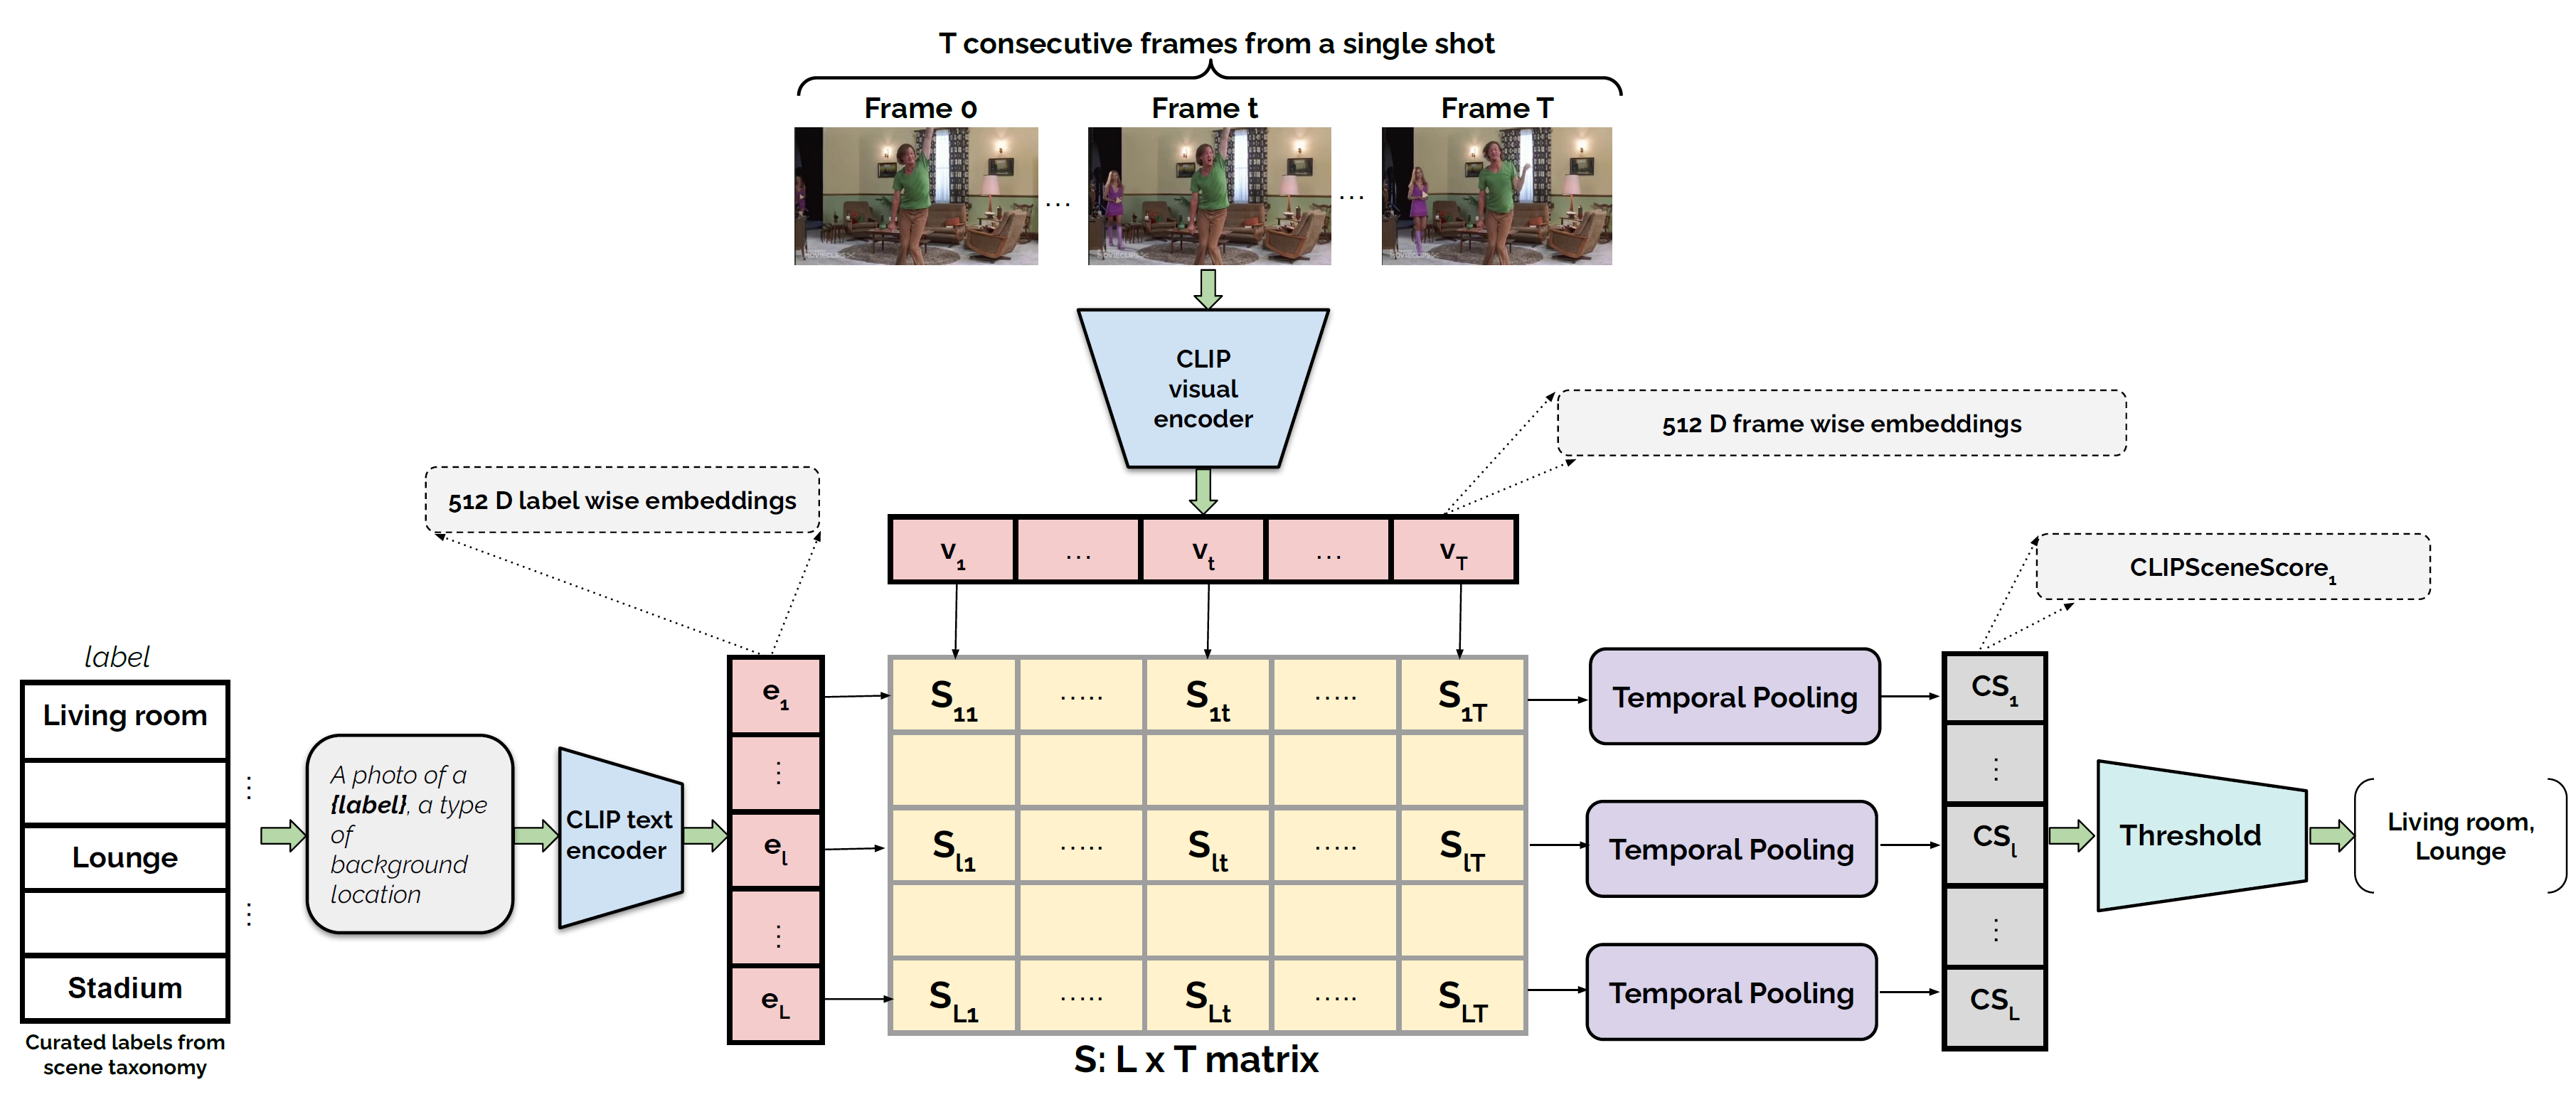
\includegraphics[width=\textwidth]{figures/MovieCLIP_tagging_image.png} %0.8\textwidth
\caption{Overview schematic of the prompt-based visual scene labeling of movie shot using CLIP's visual and text encoders. $S$ is the similarity matrix where entry $S_{lt}$ refers to similarity values between textual embedding $e_{l}$ and visual embedding $v_{t}$.}
\label{clip tagging}
\end{figure*}
In this section, we describe how CLIP \cite{CLIP} can be used to associate visual scene labels with individual movie shots. Based on prompt engineering designs considered by GPT3 \cite{GPT3}, addition of contextual phrases like \textit{\textbf{``a type of pet"}} or \textit{\textbf{``a type of food"}} in the prompts provides additional information for CLIP for zero shot classification. In a similar vein, we consider the visual scene specific prompt: \textit{\textbf{``A photo of a \{label\}, a type of background location"}} to tag individual frames in video clips with labels from our scene taxonomy. If a shot contains $T$ frames, we utilize CLIP's visual encoder to extract frame-wise visual embeddings $v_{t}(t=1,...,T)$. For each of the individual scene labels in our taxonomy, we utilize CLIP's text encoder to extract embeddings $e_{l} (l=1,2,...,L)$ for the background-specific prompts 
We use the label-wise (prompt-specific) text and frame-wise visual embeddings to obtain a similarity score matrix $S$, whose entries $S_{lt}$ are computed as follows:
\begin{equation}\label{simmatrixscore}
    S_{lt}=\frac{e_{l}^{T}v_{t}}{\lVert e_{l}  \rVert_{2}  \lVert v_{t} \rVert_{2}}
\end{equation}
We compute an aggregate shot-specific score for individual scene labels by temporal average pooling over the similarity matrix $S_{lt}$, since the visual content within a shot remains fairly unchanged. The computation of shot-specific score called $\texttt{CLIPSceneScore}_{\texttt{l}}$ for $l$th visual scene label is shown in Eq.~\ref{score pooling}.
Overall workflow of the process is illustrated in Fig \ref{clip tagging}.
\begin{equation}
    \texttt{CLIPSceneScore}_{\texttt{l}}=\frac{\sum_{t=0}^{T}(S_{lt})}{T}
    \label{score pooling}
\end{equation}

\subsection{Prompt design choices}
In terms of prompt designs, we consider the following templates customized for generic background information:
\begin{itemize}
    \item \textit{A photo of \{\}, a type of background location}
    \item \textit{A photo of \{\}, a type of location}
\end{itemize}
Since multiple shots consider people in focus, we also consider the following people-centric prompt templates:

\begin{itemize}
    \item \textit{People at \{\}, a type of background location}
    \item \textit{People at \{\}, a type of location}
\end{itemize}

As shown in Fig \ref{Combined Prompt Setup}, the prompts associated with generic background information tend to perform better in terms of associating visual scene labels to movie shots with higher confidence, when compared with people-centric prompts. Further inclusion of the contextual phrase \textit{"a type of background location"} tends to perform better than \textit{"a type of location"} in associating top-1 visual scene labels with higher $\texttt{CLIPSceneScore}$ values. When people-centric prompts are used, the CLIP based labeling scheme can result in incorrect associations like interrogation room in Fig \ref{Combined Prompt Setup} (a) and cockpit in Fig \ref{Combined Prompt Setup} (c). Hence we consider \textit{A photo of \{\}, a type of background location} as our final prompt choice.
\begin{figure*}[h!]
    \centering
    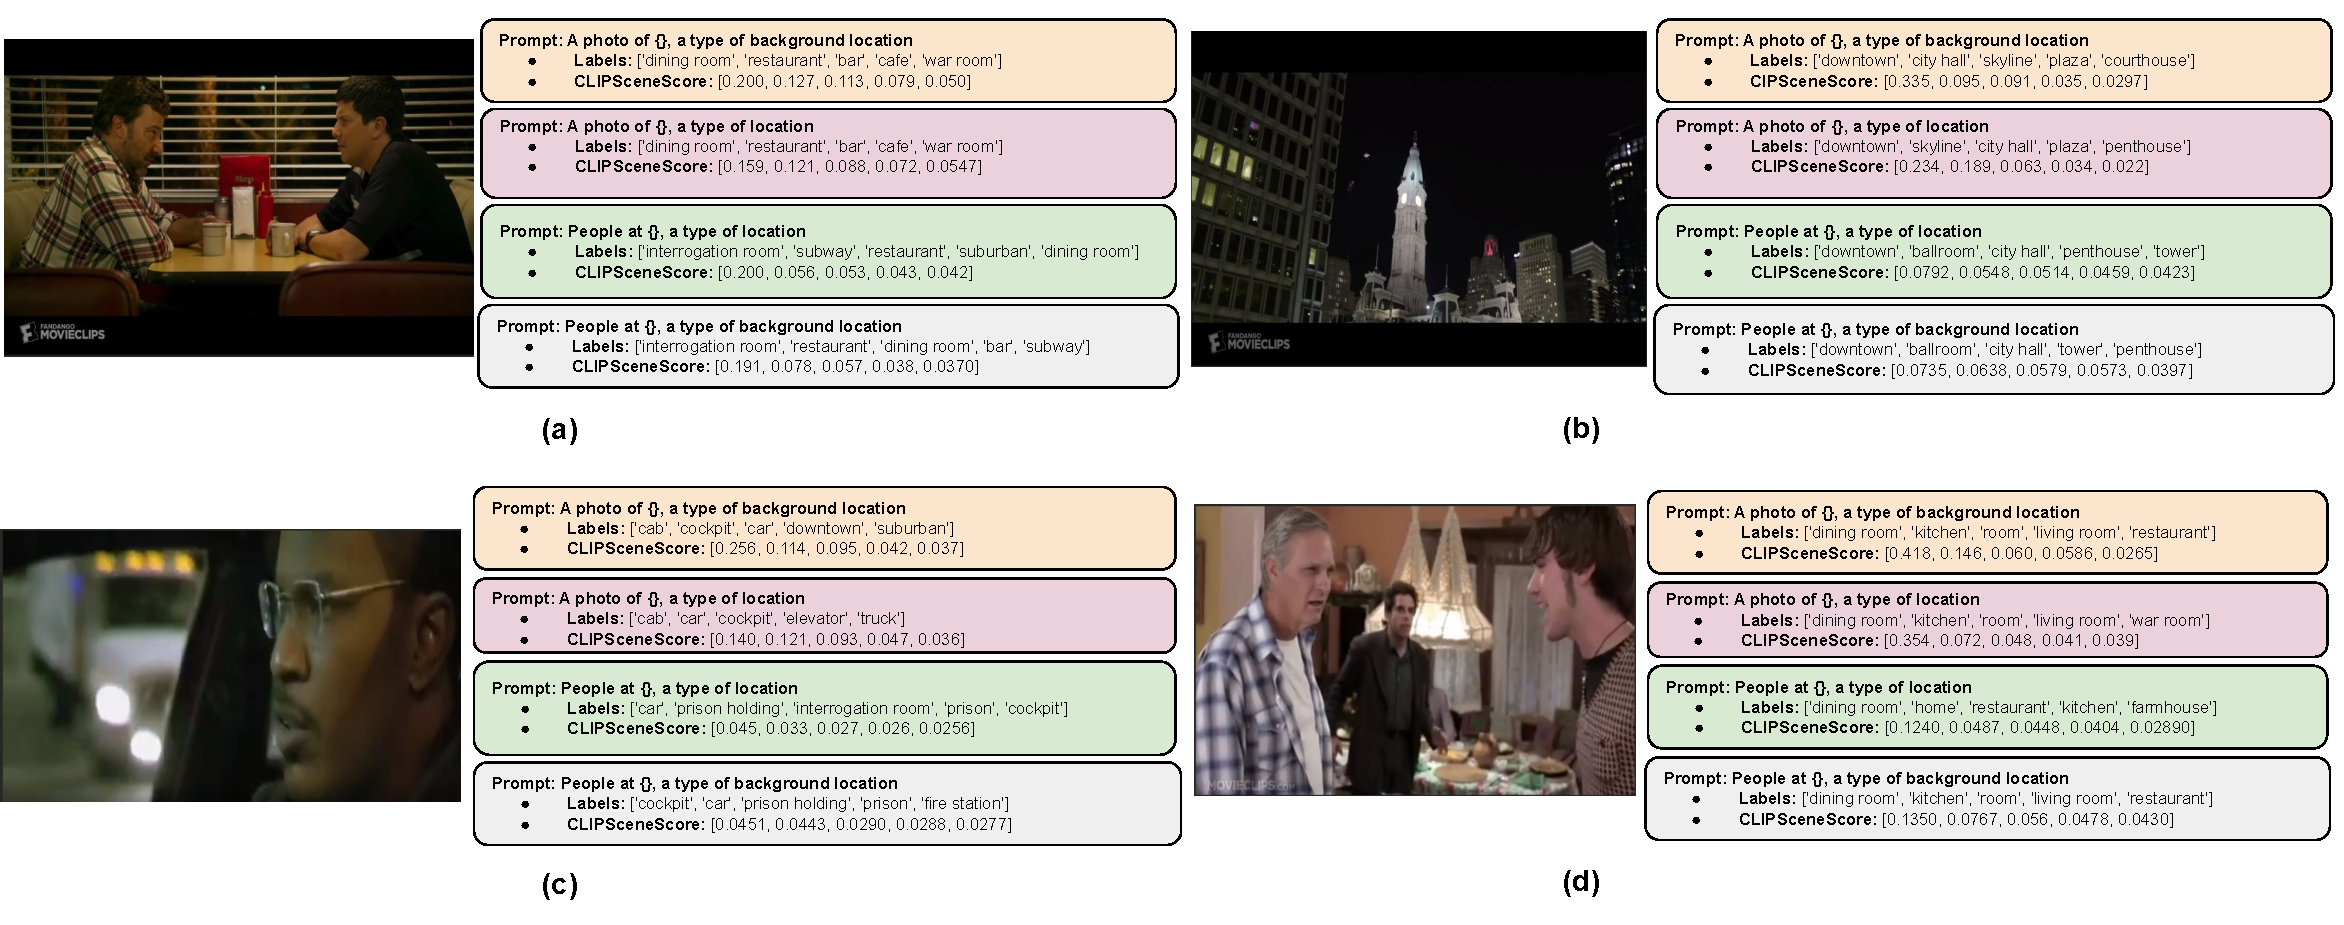
\includegraphics[width=\textwidth]{figures/Prompt_Design_combined_updated.pdf}
    \caption{Examples of various prompt templates and associated CLIPSceneScores for top-k visual scene labels. Here k=5}
    \label{Combined Prompt Setup}
\end{figure*}

\subsection{Analysis of CLIP tagging}

\subsubsection{Qualitative examples}

\begin{figure}[h!]
\centering
\subfloat[]{%
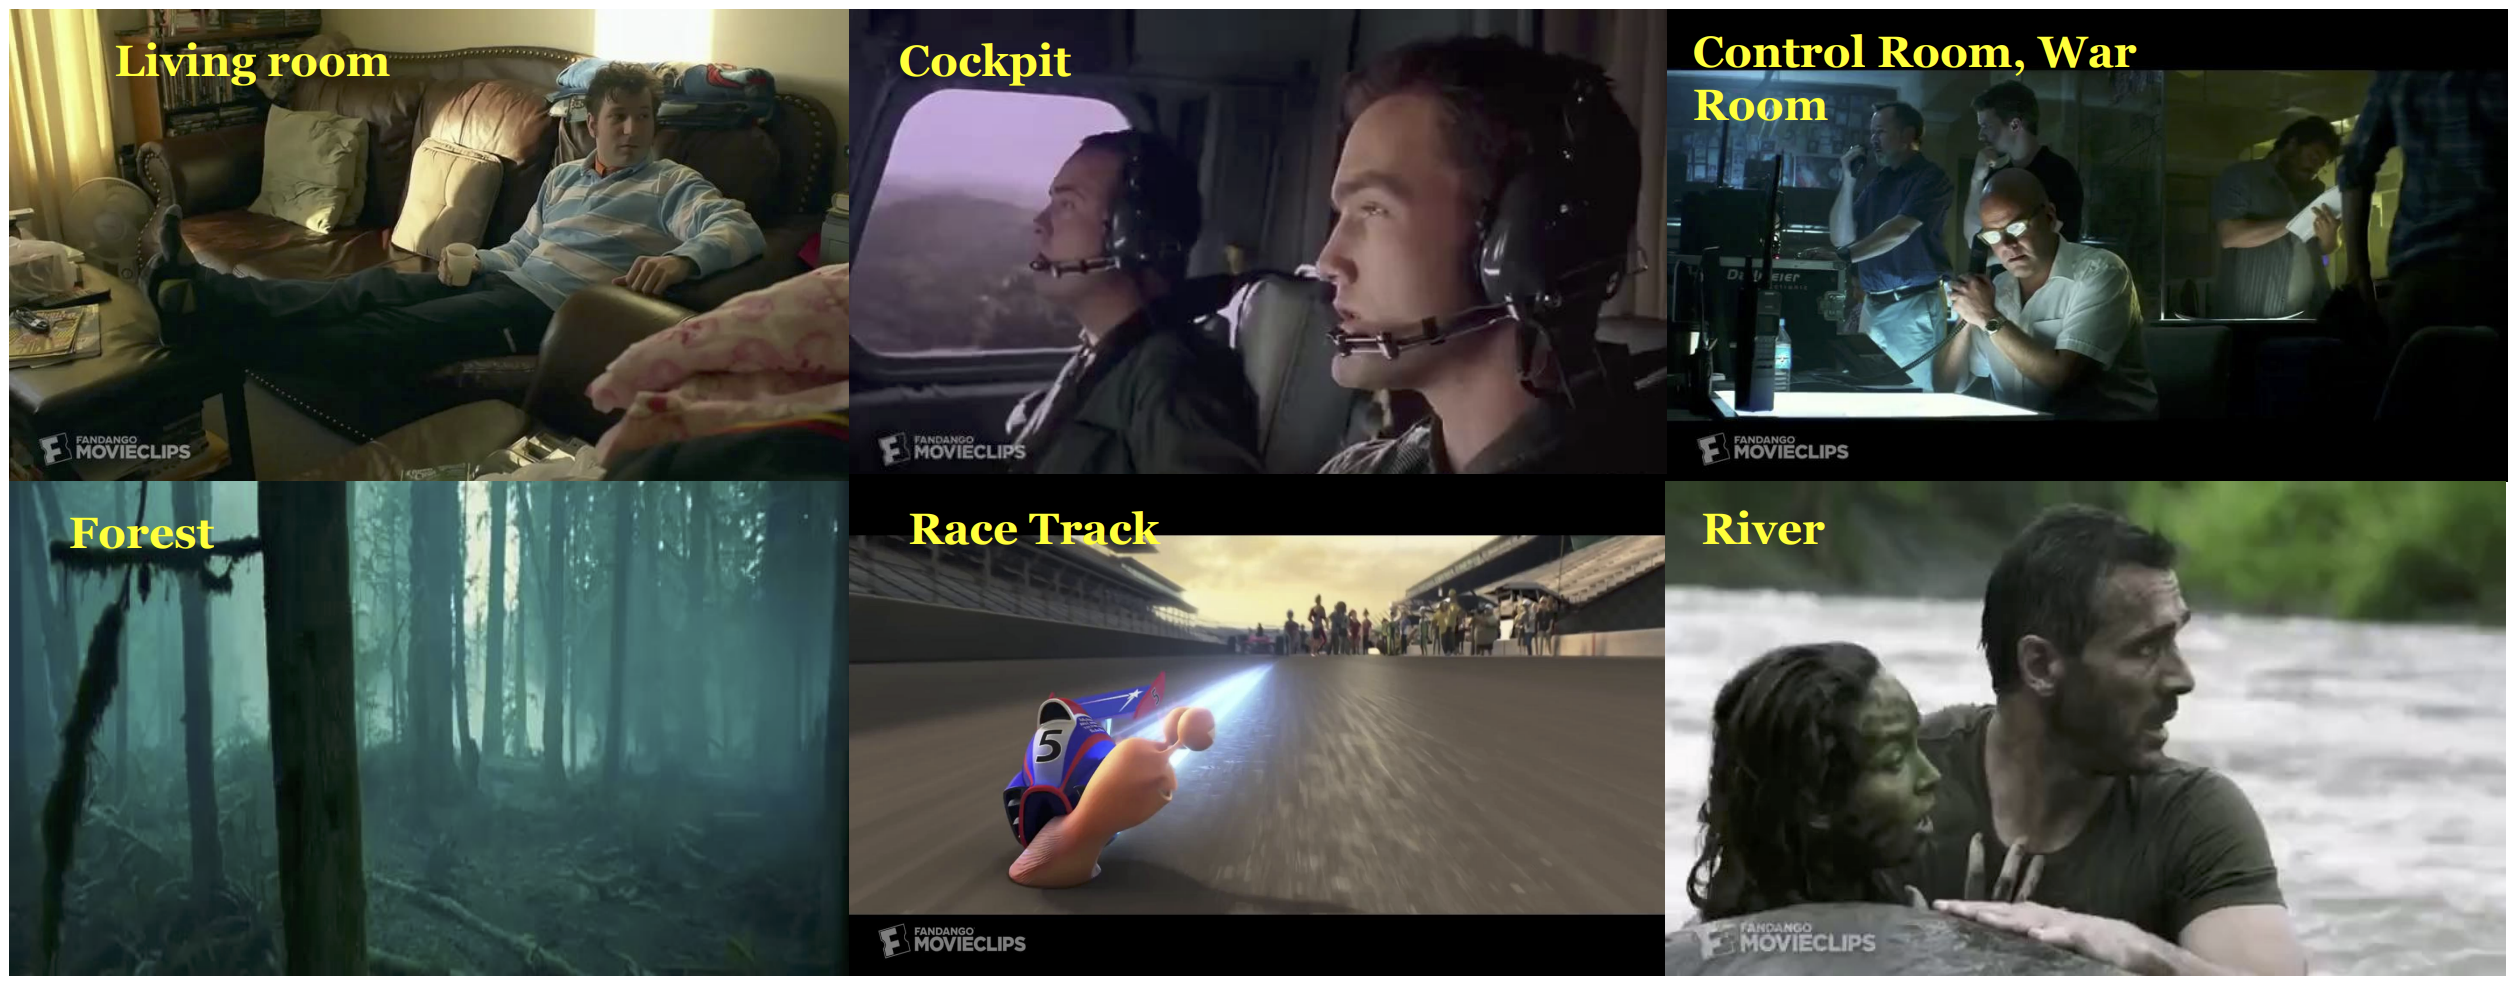
\includegraphics[width=0.5\textwidth]{figures/CLIP_high_confidence.png}% 
\label{clip high conf}
}
\subfloat[]{%
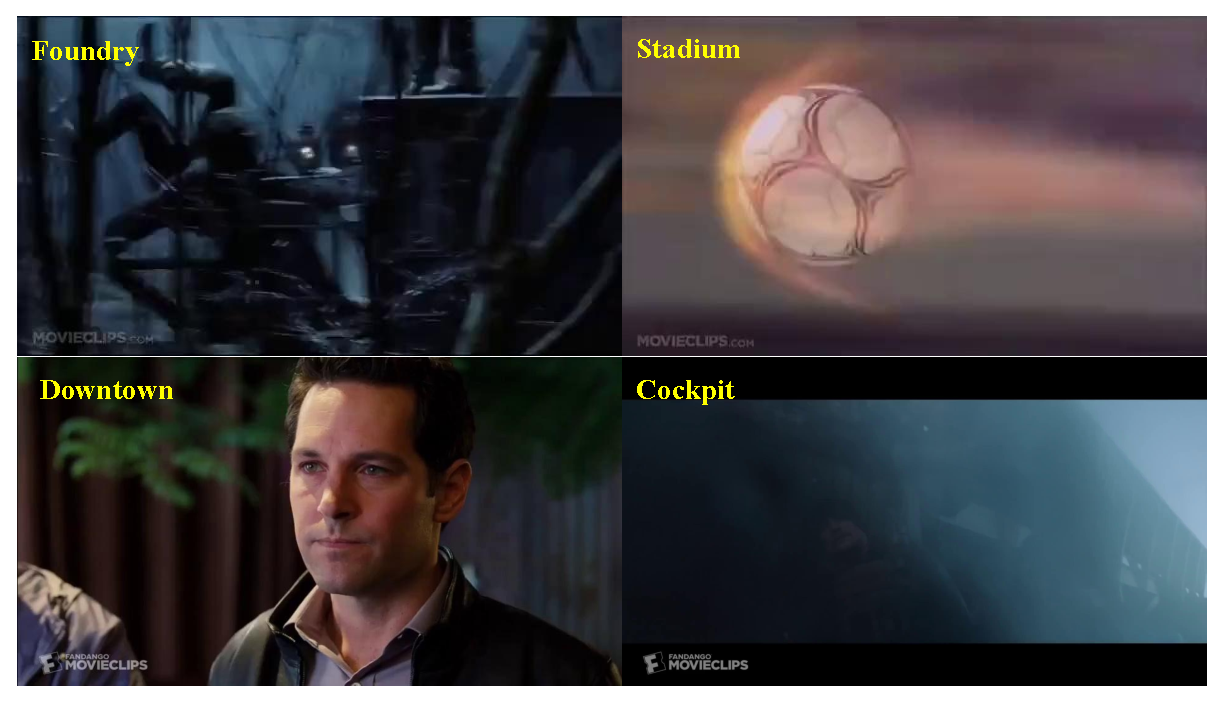
\includegraphics[width=0.5\textwidth]{figures/CLIP_bad_samples_v2.pdf}%
\label{clip low conf}
}
\caption{(a) Sample frames from the movie shots labeled by CLIP with high confidence (\texttt{CLIPSceneScore} $\geq$ 0.6 and Labels shown in yellow) (b) Sample frames from the movie shots tagged by CLIP with low confidence (Labels shown in yellow).}
\label{combined slulgline and image datasets}
\end{figure}
As shown in Fig \ref{clip high conf}, CLIP performs well when distinctive elements of visual scene are present like background objects in indoor locations (living room) or appearance-based cues (green color background for forests).
For example in  \ref{clip high conf}, the presence of airplane windows indicates that the associated visual scene label with the given movie shot is cockpit. However, for shots involving blurry motion or absence of background information due to the close up of the involved characters, CLIP's confidence in associating visual scene labels is low (Fig \ref{clip low conf}).
\\
\textbf{Genre-wise association:} 
\begin{figure}[h!]
    \centering
    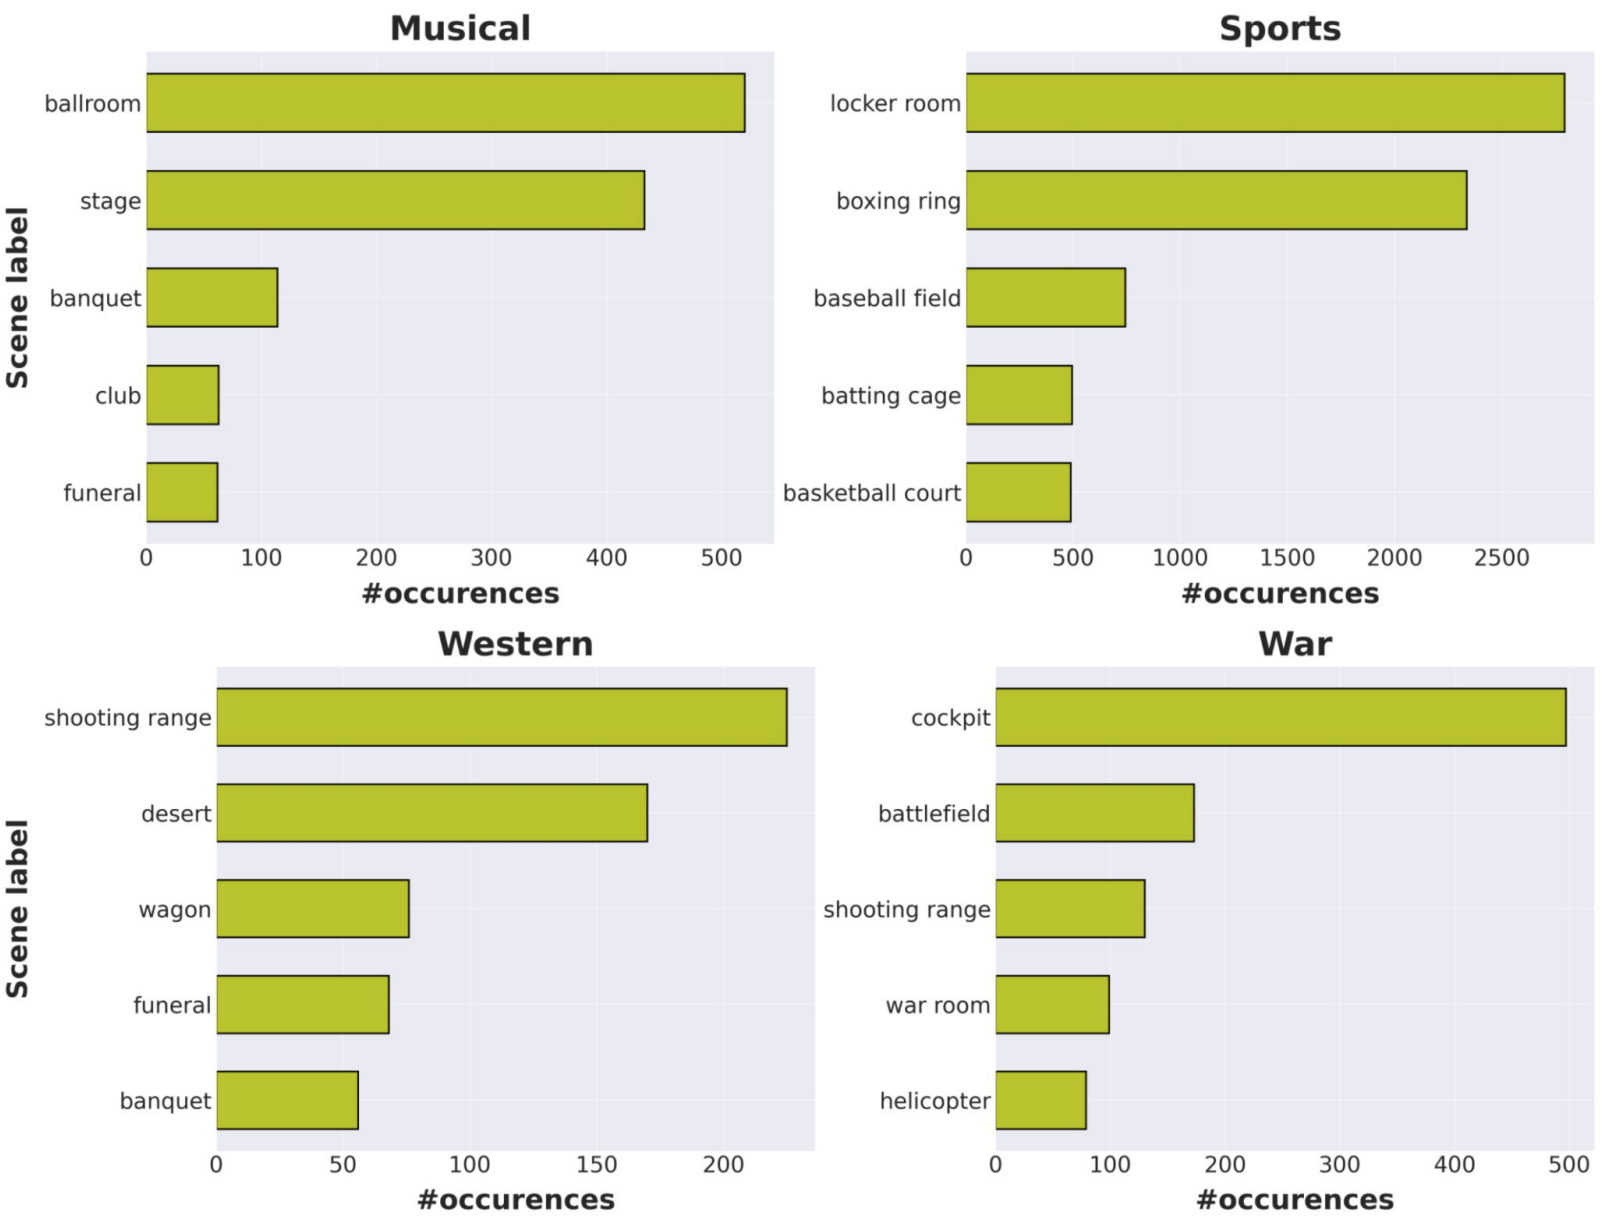
\includegraphics[width=0.8\columnwidth]{figures/genre_wise_distribution_plots_clip_label.png}
    \caption{Genre-wise distribution of different scene labels. For each genre, the top-5 scene labels are shown in terms of the number of occurrences in the top-1 label provided by CLIP \cite{CLIP} for shots in the MovieCLIP dataset. Threshold for confidence score of top-1 label = 0.4}
    \label{genre distribution}
\end{figure}
We consider those shots whose top-1 $\texttt{CLIPSceneScore}$ values are greater than or equal to 0.4 and show the top-5 scene labels in terms of occurrences for certain genres like \textit{western}, \textit{sport}, \textit{war} and \textit{musical}.  From Fig \ref{genre distribution}, we can see that relevant scenes are associated with genres through CLIP's labeling scheme. Some notable examples include \{shooting range, desert\} for \textit{western}, \{locker room, boxing ring\} for \textit{sport}, \{ballroom, stage\}  for \textit{musical} and \{cockpit, battlefield\} for \textit{war}.

\subsubsection{Shot type distribution:}
We analyze the distribution of shot types in terms of scale for samples extracted from Condensed Movies dataset \cite{bain2020condensed}. We consider the shot scale type taxonomy in MovieShots \cite{rao2020unified} dataset as follows:

\begin{itemize}
    \item \textbf{Long shot (LS):} Shot taken from long distance like quarter of a mile and having least person close up.
    \item \textbf{Full shot (FS):} Shot showing the entire human body.
    \item \textbf{Medium shot (MS):} Shot showing the humans from knees or waist up.
    \item \textbf{Close-up shot (CS):} Shot focussed on a small segment like face of a person.
    \item \textbf{Extreme close-up shot (ECS):} Shot showing smaller regions like image of eye or mouth.
\end{itemize}

We use the samples in the MovieShots dataset to train a 2-layer LSTM \cite{lstm} network (hidden dimension = 512) to classify between 5 scale classes. For individual shots, we extract frame-wise features from pretrained ViT-B/16 \cite{dosovitskiy2020vit} network at 4 fps for inputs to the LSTM network. For training, validation and testing we use a split of 23557, 6764, and 3332 shots. We use the trained model to predict the shot scale labels for the samples in the MovieCLIP dataset.
\par 
From Figure \ref{shot scale distribution} (a), we can see that for low-confidence shots in MovieCLIP dataset having top-1 \texttt{CLIPSceneScore} $<=0.2$, significant proportion (86\%) have person close-up ranging from moderate (\textbf{MS}) to very high (\textbf{ECS}). When combined, Close-up (\textbf{CS}) and extreme close-up (\textbf{ECS}) shots constitute 50\% of total samples having top-1 \texttt{CLIPSceneScore} $<=0.2$. However for high confidence shot samples in MovieCLIP, whose top-1 \texttt{CLIPSceneScore} values are greater than 0.4, the combined share of \textbf{CS} and \textbf{ECS} scale labels decreases to 24\%. Further, the combined share of \textbf{FS} and \textbf{LS} rises from 14\% in Fig \ref{shot scale distribution} (a) to 35\% in Fig \ref{shot scale distribution} (b). 
This indicates that a major share of the shot samples having low  \texttt{CLIPSceneScore} values have high(\textbf{CS}) to very high (\textbf{ECS}) person close-up. Whereas the increasing share of \textbf{FS} and \textbf{LS} scale labels in Fig \ref{shot scale distribution} shows that CLIP needs more background information in the shots to tag visual scenes with high confidence.
\begin{figure*}[h!]
\centering
\subfloat[]{%
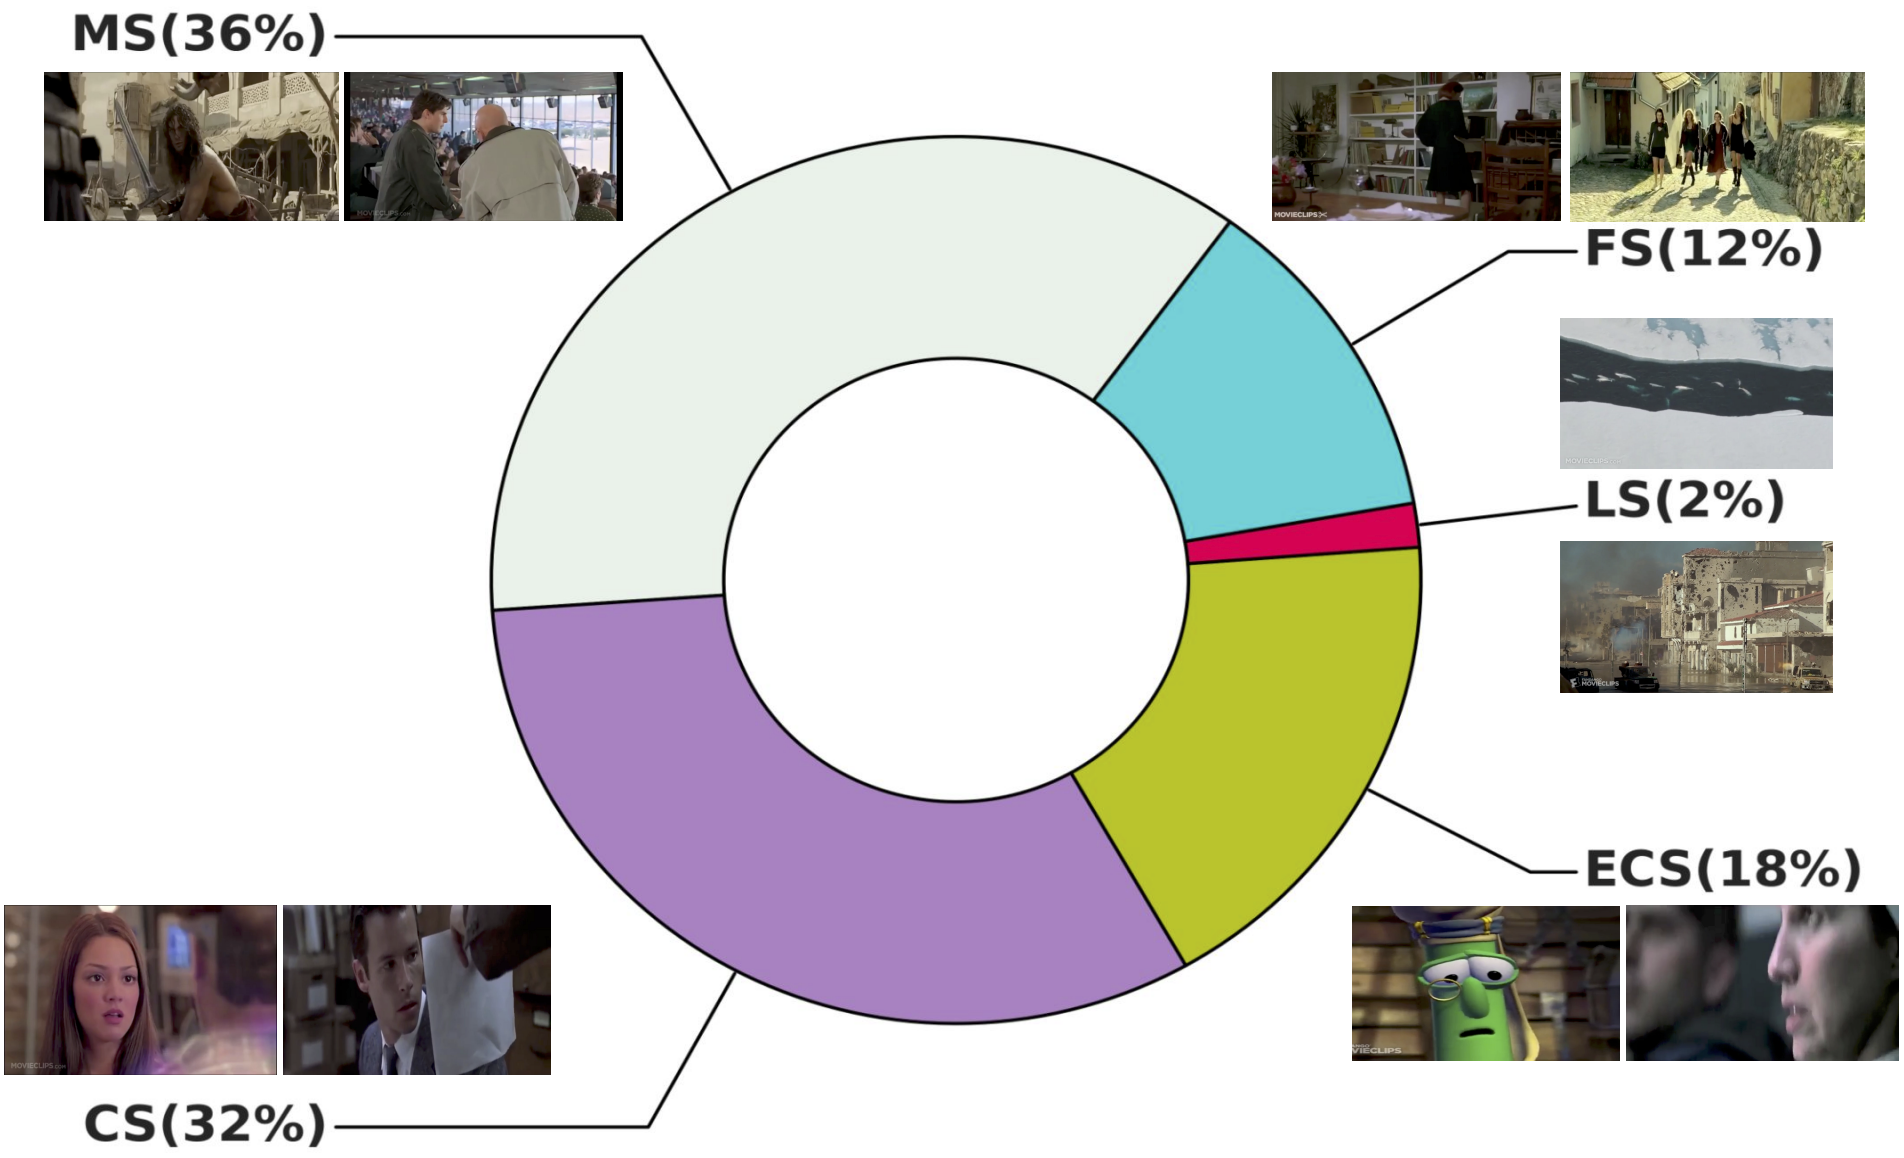
\includegraphics[width=0.45\textwidth]{figures/wedge_plot_low_threshold_sample.png}
\label{}
}\hfill
\subfloat[]{%
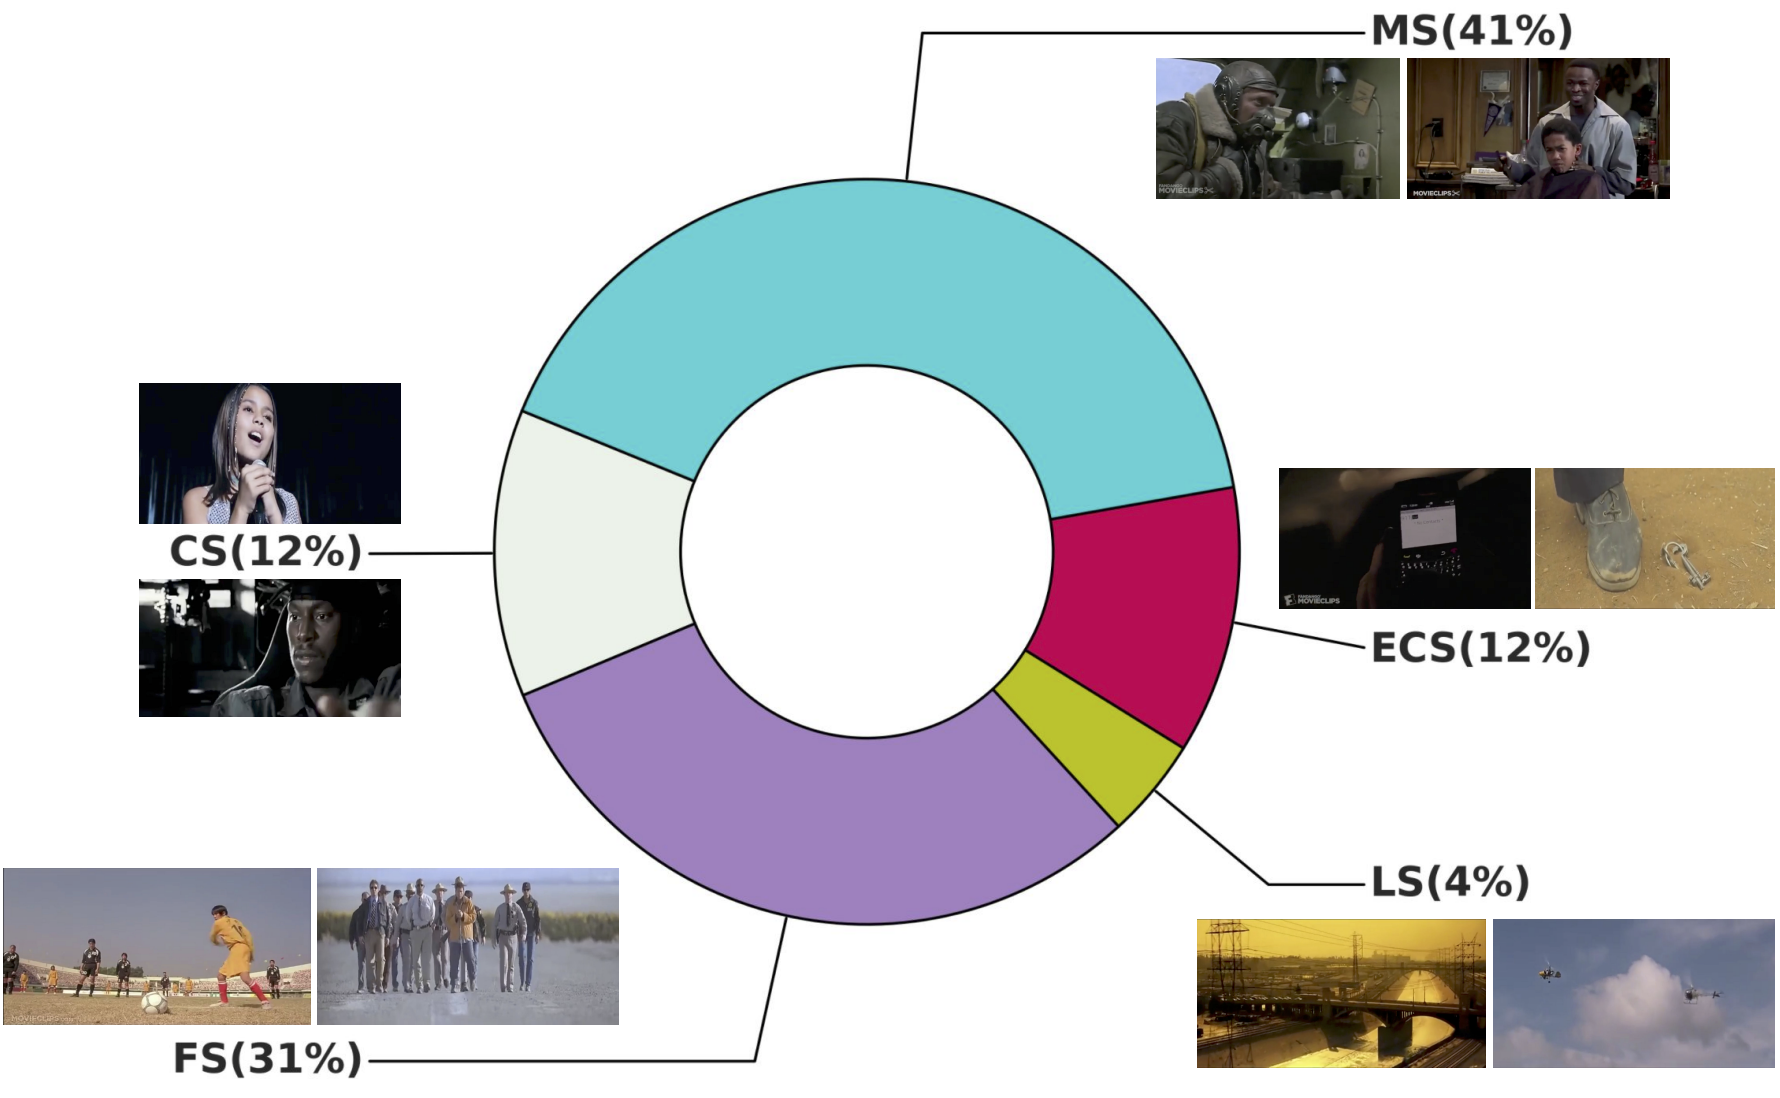
\includegraphics[width=0.5\textwidth]{figures/wedge_plot_high_threshold_shot_sample.png}
\label{clip low conf}
}
\caption{(a) Distribution of predicted scale labels for shots (N=745059) in MovieCLIP dataset having top-1 \texttt{CLIPSceneScore} $<=0.2$(b) Distribution of predicted scale labels for shots (N=107420) in MovieCLIP dataset having top-1 \texttt{CLIPSceneScore} $>=0.4$ and top-k \texttt{CLIPSceneScore} $>=0.1$ (\texttt{k=2,3,4,5}). Scale labels include : \textbf{ECS}: Extreme Close-up shot, \textbf{CS}: Close-up shot, \textbf{MS}: Medium shot, \textbf{LS}: Long shot, \textbf{FS}: Full shot.}
\label{shot scale distribution}
\end{figure*}
\subsection{Quality estimation through human verification}
In order to estimate the reliability of the top-k labels provided by CLIP for movie shots, we conducted a verification task on Amazon Mechanical Turk. We provided a pool of annotators with a subset of 2393 movie shots from VidSitu \cite{Sadhu_2021_CVPR} dataset, along with top-5 scene labels. As shown in Fig \ref{mturk experiment},  if none of the scene labels appear relevant for the given movie shot, the annotators choose the \textbf{Not relevant} option.  After the human verification experiment is complete, we discard the shot samples with no agreements and obtain evaluation data consisting of 1883 shot samples. We also use the LSTM model pretrained on MovieShots dataset to predict shot types for samples that have no agreements with human experts. The distribution of shot-wise predictions from the trained LSTM model is shown in Fig \ref{shot_type_distribution}. We can see that 80\% of shots having no agreements with human annotations belong to the shot categories having moderate (MS) to very high person closeup (ECS). 
\begin{figure*}[h!]
    \centering
    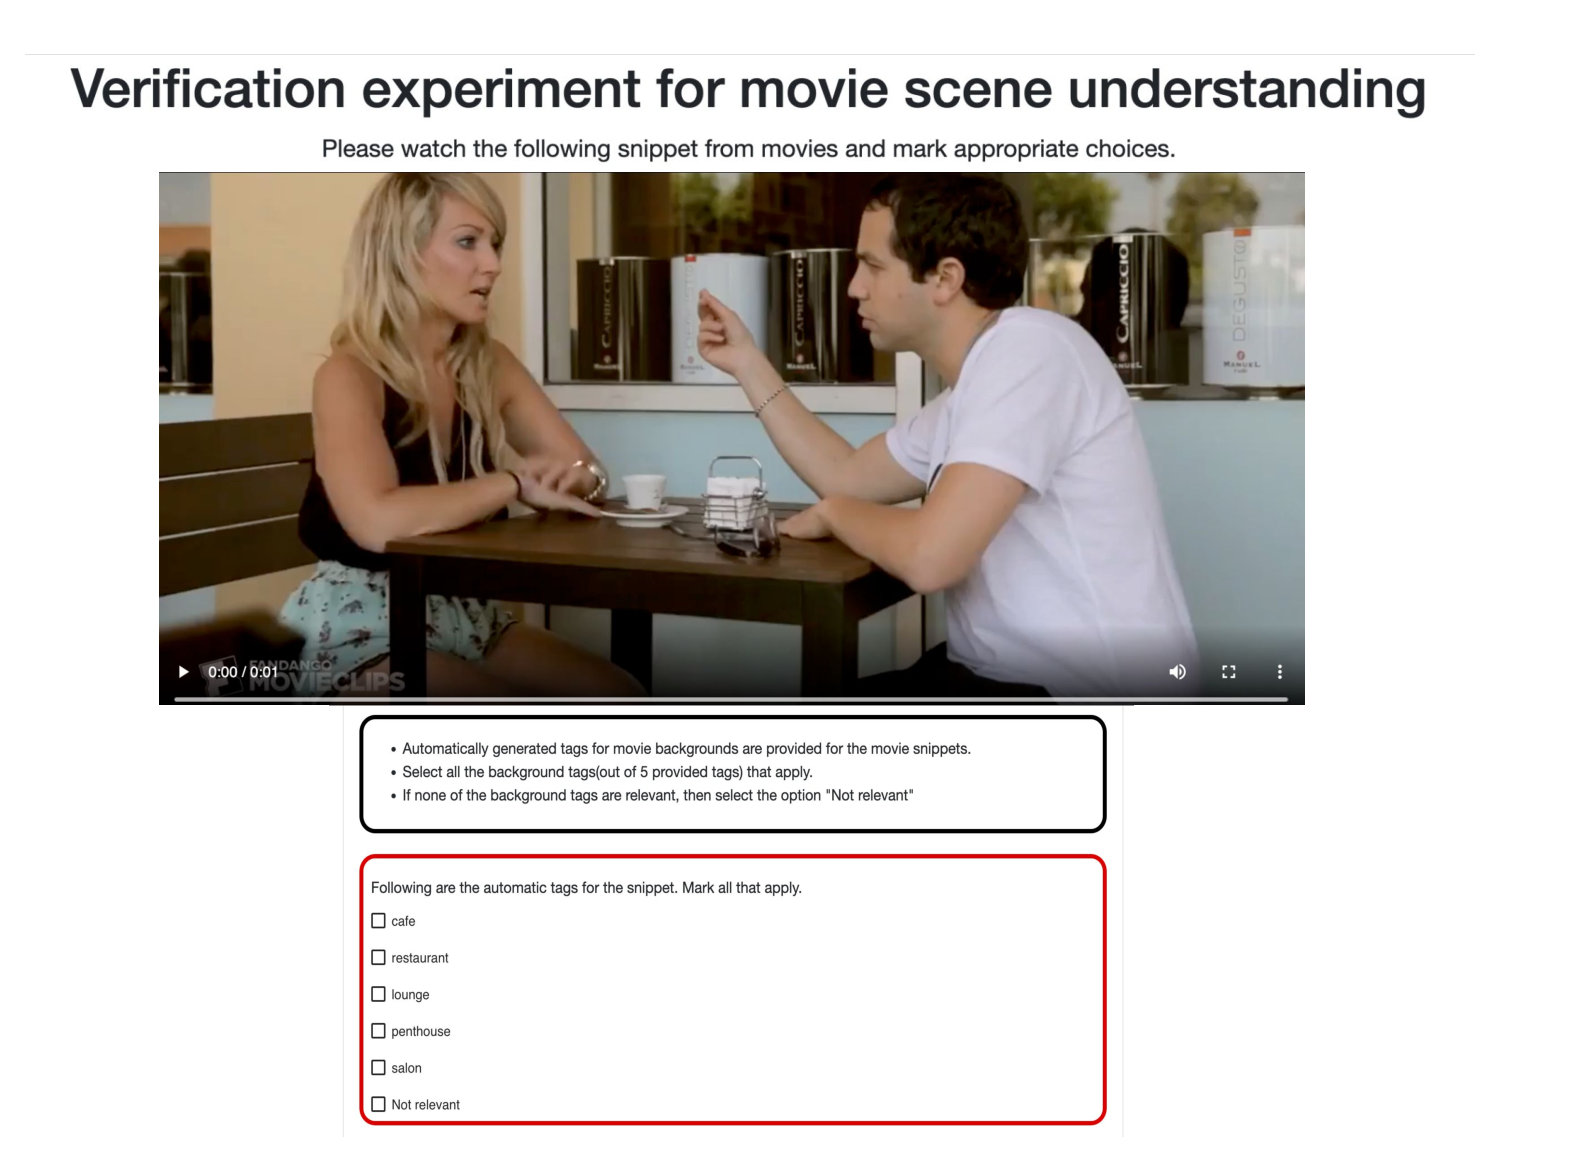
\includegraphics[width=0.8\textwidth]{figures/verification_experiment.pdf}
    \caption{Schematic design of the mturk experiment used for human verification of visual scenes.}
    \label{mturk experiment}
\end{figure*}
\begin{figure}
    \centering
    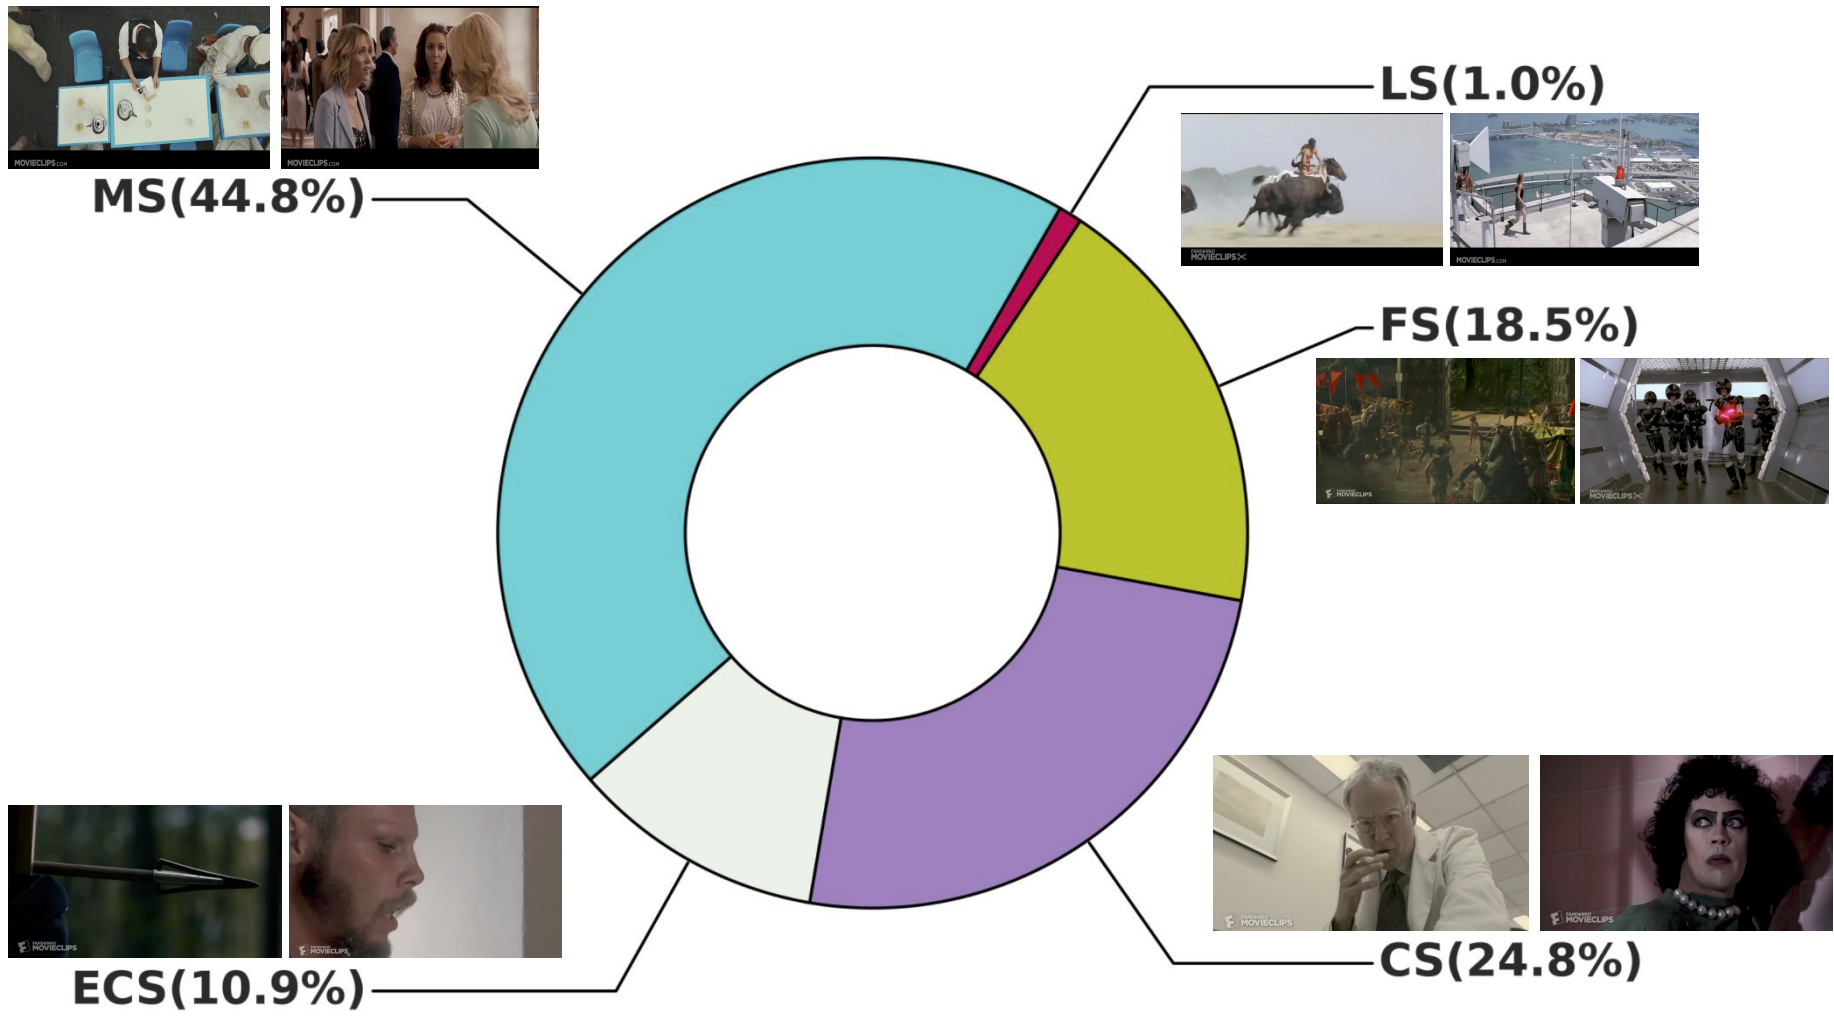
\includegraphics[width=0.8\textwidth]{figures/Shot_type_distribution_discarded_shots.png}
    \caption{Distribution of shot scale predictions among the shots having no agreements between human annotators and CLIP's labeling scheme. \textbf{ECS}: Extreme Close-up shot, \textbf{CS}: Close-up shot, \textbf{MS}: Medium shot, \textbf{LS}: Long shot, \textbf{FS}: Full shot}
    \label{shot_type_distribution}
\end{figure}

\section{Experiments and Results:}

\subsection{Experimental Setup}
For training and validation purposes, we retain those shot samples whose top-1 $\texttt{CLIPSceneScore}$ is greater than or equal to 0.4 (approx 75 percentile), resulting in a clean subset. After top-1 filtering, we also consider labels from top-k (k = 2 to 5) whose $\texttt{CLIPSceneScore}$ is greater than 0.1 to associate multiple labels per sample.
This results in a set of \textbf{107k} samples with train, val and test split of \textbf{73.8k}, \textbf{23.2k} and \textbf{10.3k} having non-intersecting set of ids with the human-verified evaluation set. Approximately \textbf{38.4\%} of the dataset is multi-label, covering 150 scene classes out of 179 in the curated scene taxonomy. 
All the related experiments were conducted using the Pytorch\cite{Pytorch} framework using 4 T4 NVIDIA GPUs. For training the respective models, we use binary cross entropy loss function. For evaluation, we use \textbf{mean average precision (mAP)} and \textbf{Pearson correlation} (averaged across samples) as metrics.


\subsection{Visual scene recognition - Movies}
\textbf{Frame-wise aggregation models:} For frame-wise aggregation, we extract dense embeddings from individual shots at 4fps. We use two sets of embeddings: 512 dim embedding from Resnet18 \cite{He2015} pretrained on Places2 dataset and 768 dim embedding from ViT-B/16 \cite{dosovitskiy2020vit} model pretrained on Imagenet \cite{Deng2009ImageNetAL}.
Following feature extraction, we perform temporal aggregation using LSTM \cite{lstm} with 2 layers and hidden dimension of 512.
\\
\textbf{3D Convolutional network models:} 
We use I3D\cite{i3d}, R(2+1)D \cite{r2plus1d}, Slowfast \cite{feichtenhofer2019slowfast} as baseline 3D convolutional models in multi-label setup. I3D\cite{i3d} and Slowfast\cite{feichtenhofer2019slowfast} models have a Resnet50\cite{He2015} backbone whereas R(2+1)D \cite{r2plus1d} has a Resnet34\cite{He2015} backbone. All the models are initialized from Kinetics400 \cite{kinetics400} pretrained weights. For finetuning I3D\cite{i3d} and Slowfast\cite{feichtenhofer2019slowfast}, we use SGD with learning rates in $\{0.1,1e-3\}$ and weight decay of 1e-4. For R(2+1)D \cite{r2plus1d} we use Adam \cite{Kingma2015AdamAM} with learning rate 1e-4. Batch sizes for the models are varied between 16 and 32. \\
\textbf{Video Transformer models:}
For video transformer models, we consider the base TimeSformer model \cite{Bertasius2021IsSA} that considers 8 frames (224 x 224) as inputs. For finetuning TimeSformer \cite{Bertasius2021IsSA} model, we use SGD with learning rate 5e-3 and weight decay of 1e-4 and batch size of 8. For better speed-accuracy tradeoff we use the Video Swin Transformer model \cite{liu2021video}, \cite{liu2021Swin} called Swin-B with clip size of 32 frames (224 x 224) as inputs. For finetuning we use AdamW \cite{AdamW} optimizer with learning rate 1e-4 and Cosine Annealing with batch size of 32. 
\par 
Based on the results in Table \ref{visual movie models}, we can see that 2-layer LSTM model trained using features from Imagenet-21K pretrained ViT-B/16 performs better compared to features extracted using Resnet-18 model pretrained on Places2 dataset. This shows that features from Places2 pretrained models might not be optimal for scene recognition in the movie domain.
In terms of end-to-end models, video transformers, including TimeSformer and Swin-B models outperform 3D convolutional models. Swin-B model performs better than other models by obtaining an average correlation of \textbf{0.497} and mean average precision of \textbf{44.4}.
\begin{table}[h!]
\centering
\resizebox{0.7\columnwidth}{!}{
\begin{tabular}{|cccc|}
\hline
\multicolumn{4}{|c|}{\textbf{Frame wise aggregation}}                                                                         \\ \hline
\multicolumn{1}{|c|}{Model}                & \multicolumn{1}{c|}{Features}         & \multicolumn{1}{c|}{mAP}   & Correlation \\ \hline
\multicolumn{1}{|l|}{LSTM (512, 2 layers)} & \multicolumn{1}{c|}{Places2 (4 fps)}  & \multicolumn{1}{c|}{24.15} & 0.29        \\ \hline
\multicolumn{1}{|l|}{LSTM (512, 2 layers)} & \multicolumn{1}{l|}{ViT-B/16 (4 fps)} & \multicolumn{1}{c|}{43.10} & 0.42        \\ \hline
\multicolumn{4}{|c|}{\textbf{3D convolutional networks}}                                                                      \\ \hline
\multicolumn{1}{|c|}{Model}                & \multicolumn{1}{c|}{Features}         & \multicolumn{1}{c|}{mAP}   & Correlation \\ \hline
\multicolumn{1}{|c|}{SlowFast (R50) \cite{feichtenhofer2019slowfast}}       & \multicolumn{1}{c|}{NA}               & \multicolumn{1}{c|}{25.80}      &   0.402         \\ \hline
\multicolumn{1}{|c|}{R(2+1)D (R34) \cite{r2plus1d} }        & \multicolumn{1}{c|}{NA}               & \multicolumn{1}{c|}{26.73} & 0.40        \\ \hline
\multicolumn{1}{|c|}{I3D (R50) \cite{i3d}}            & \multicolumn{1}{c|}{NA}               & \multicolumn{1}{l|}{13.33} & 0.26        \\ \hline
\multicolumn{4}{|c|}{\textbf{Video Transformers}}                                                                             \\ \hline
\multicolumn{1}{|c|}{TimeSformer \cite{Bertasius2021IsSA}}          & \multicolumn{1}{c|}{NA}               & \multicolumn{1}{l|}{36.87} & 0.46        \\ \hline
\multicolumn{1}{|c|}{\textbf{Swin-B} \cite{liu2021video}}             & \multicolumn{1}{c|}{\textbf{NA}}              & \multicolumn{1}{c|}{\textbf{44.4}}  & \textbf{0.497}       \\ \hline
\end{tabular}}
\vspace{1mm}
\caption{Mean average precision (\textbf{mAP}) and average Spearman correlation of different models on human-verified evaluation set (N=1883 shots). NA: End-to-end models used instead of features. For 3D conv models, the backbone network is mentioned inside brackets. }
\label{visual movie models}
\end{table}
\subsection{Downstream tasks}
\subsubsection{Visual scene recognition - web videos}
We also explore knowledge transfer from models finetuned on MovieCLIP by evaluating performance on downstream multi-label scene classification with HVU dataset \cite{diba_large_2020}. For training and evaluation, we use 251k and 16k videos with 248 scene labels. We extract 1024 dim features from the best performing Swin-B model in Table \ref{visual movie models}.
We train 3 layer fully connected models on the respective features with the following configuration:\\
\textit{$M_{scene}$}: $\textbf{INP}[1024]\rightarrow{}\textbf{FC}[4096],\textbf{DO}(0.2)
\rightarrow{}\textbf{FC}[4096] \rightarrow{}\textbf{FC}[248]$\\
Here \textbf{FC} refers to a fully connected layer, and \textbf{DO} refers to dropout.
From Table \ref{HVU}, we can see that ${M_{scene}}$ exhibits better performance when compared to existing end-to-end models trained on HVU.
\begin{table}[h!]
\centering
\begin{tabular}{|c|c|}
\hline
\textbf{Model}                                     & \textbf{mAP} \\ \hline
3D-ResNet \cite{diba_large_2020}                                &   50.6  \\ \hline 
3D-STCNet  \cite{diba_large_2020}                            &  51.9   \\ \hline
HATNet  \cite{diba_large_2020}                              &  55.8   \\ \hline
${M_{scene}}$ &  55.92   \\ \hline
\end{tabular}
\vspace{5mm}
\caption{Mean average precision of different models on HVU dataset for multi label scene classification (248 classes). Backbone for end to end models: 3D Resnet18.}
\label{HVU}
\end{table}
\subsubsection{Multi label genre classification - movie trailers}
\begin{table*}[h!]
\centering
\resizebox{\textwidth}{!}{
\begin{tabular}{|c|c|c|c|c|c|c|c|c|c|c|c|c|c|c|}
\hline
\textbf{Model} & \textbf{Overall} & \textbf{Ac} & \textbf{Ani} & \textbf{Bio} & \textbf{Com} & \textbf{Cri} & \textbf{Drm} & \textbf{Fmy} & \textbf{Fntsy} & \textbf{Hrrr} & \textbf{Myst} & \textbf{Rom} & \textbf{ScF} & \textbf{Thrl} \\ \hline
$M_{trailer}$  & 56.14  &  62.97   &  86.51   &  14.4  &  80.77 &  49.58  &  79.58   &  74.55  &  49.59  &  50.62  &  26.83 &  45.05   &   47.99 & 61.36 \\ \hline
% FCensm $^{\ast}$         & 56.26            & 62.42       & 87.39        & 14.66        & 81.07        & 49.36        & 79.82        & 74.9         & 48.64          & 51.71         & 28.5          & 44.82        & 47.93        & 60.2          \\ \hline
C3D  \cite{DuTran}         & 53.4             & 63.8        & 91.3         & 16.2         & 82.3         & 45.1         & 71.6         & 65.3         & 54.8           & 50.8          & 28.2          & 38.3         & 21.8         & 64.8          \\ \hline
I3D  \cite{i3d}          & 38.8             & 37.2        & 51.8         & 9.2          & 72.6         & 33.9         & 67.6         & 43.6         & 39             & 22.8          & 21.3          & 34.3         & 22.6         & 48.3          \\ \hline
LSTM \cite{2019Moviescope}           & 48.4             & 47.5        & 86.8         & 12           & 79.2         & 33           & 72           & 64.5         & 54.4           & 22.7          & 24.7          & 40.4         & 36.5         & 54.8          \\ \hline
Bi-LSTM  \cite{2019Moviescope}       & 47.4             & 49.9        & 86.3         & 8.2          & 77.6         & 29.9         & 70.8         & 65.4         & 55.3           & 22.3          & 21.7          & 41.6         & 35.9         & 51.2          \\ \hline
fstVid \cite{2019Moviescope}      & 56.5             & 61.4        & 94.8         & 23.9         & 81.5         & 41.7         & 77           & 67           & 62.6           & 36.1          & 30.4          & 48.4         & 48.2         & 62            \\ \hline
fstTConv \cite{2019Moviescope} & 58.9             & 64.7        & 95.7         & 21.2         & 83.5         & 49.1         & 78.9         & 68.6         & 68.9           & 42.7          & 29.2          & 46.8         & 51           & 64.8          \\ \hline
\end{tabular}
}
\vspace{5mm}
\caption{Mean average precision of different models for multi-label genre classification (13 class) on Moviescope dataset. Except $M_{trailer}$ comparison results are reported from \cite{2019Moviescope}. Abbreviations: \textbf{Ac:} Action, \textbf{Ani:} Animation, \textbf{Bio:} Biography, \textbf{Com}: Comedy, \textbf{Cri}: Crime, \textbf{Drm}: Drama, \textbf{Fmy}: Family, \textbf{Fntsy}: Fantasy, \textbf{Hrrr}: Horror, \textbf{Myst}: Mystery, \textbf{Rom}: Romantic, \textbf{ScF}: SciFi, \textbf{Thrl}: Thriller, \textbf{fstVid}: fastVideo, \textbf{fstTConv}: fastVideo + Temporal Conv. }
\label{genre}
\end{table*}
As an additional downstream task, we consider multi-label genre classification of movie trailers in the Moviescope dataset \cite{2019Moviescope}. Out of the original set of 4927 trailers, we could access 3900 videos from YouTube. Based on the provided splits, we use 2948, 410 and 542 videos for training, validation and testing purposes, respectively. We use the 1024 dim features extracted from the best performing Swin-B model in Table \ref{visual movie models}.
%, denoted by $S_{Movie\_genre}$. 
We train 3 layer fully connected models on the respective features with the following configuration:\\
\textit{$M_{trailer}$}: $\textbf{INP}[1024]\rightarrow{} \textbf{FC}[512],\textbf{DO}(0.2)\rightarrow{}\textbf{FC}[512]\rightarrow{}\textbf{FC}[13]$\\
Even when the number of trailer videos used is a subset of the original split, $M_{trailer}$ exhibits similar genre-wise trends as other models. From Table \ref{genre}, we can see that $M_{trailer}$ shows better performance in Animation and Comedy as compared to genres like Biography and Mystery. When compared with fstTConv in Table \ref{genre}, our fully connected model $M_{trailer}$ performs slightly worse due to non-availability of entire training data. 

\subsubsection{Impact of MovieCLIP pretraining}
\begin{figure}[h!]
    \centering
    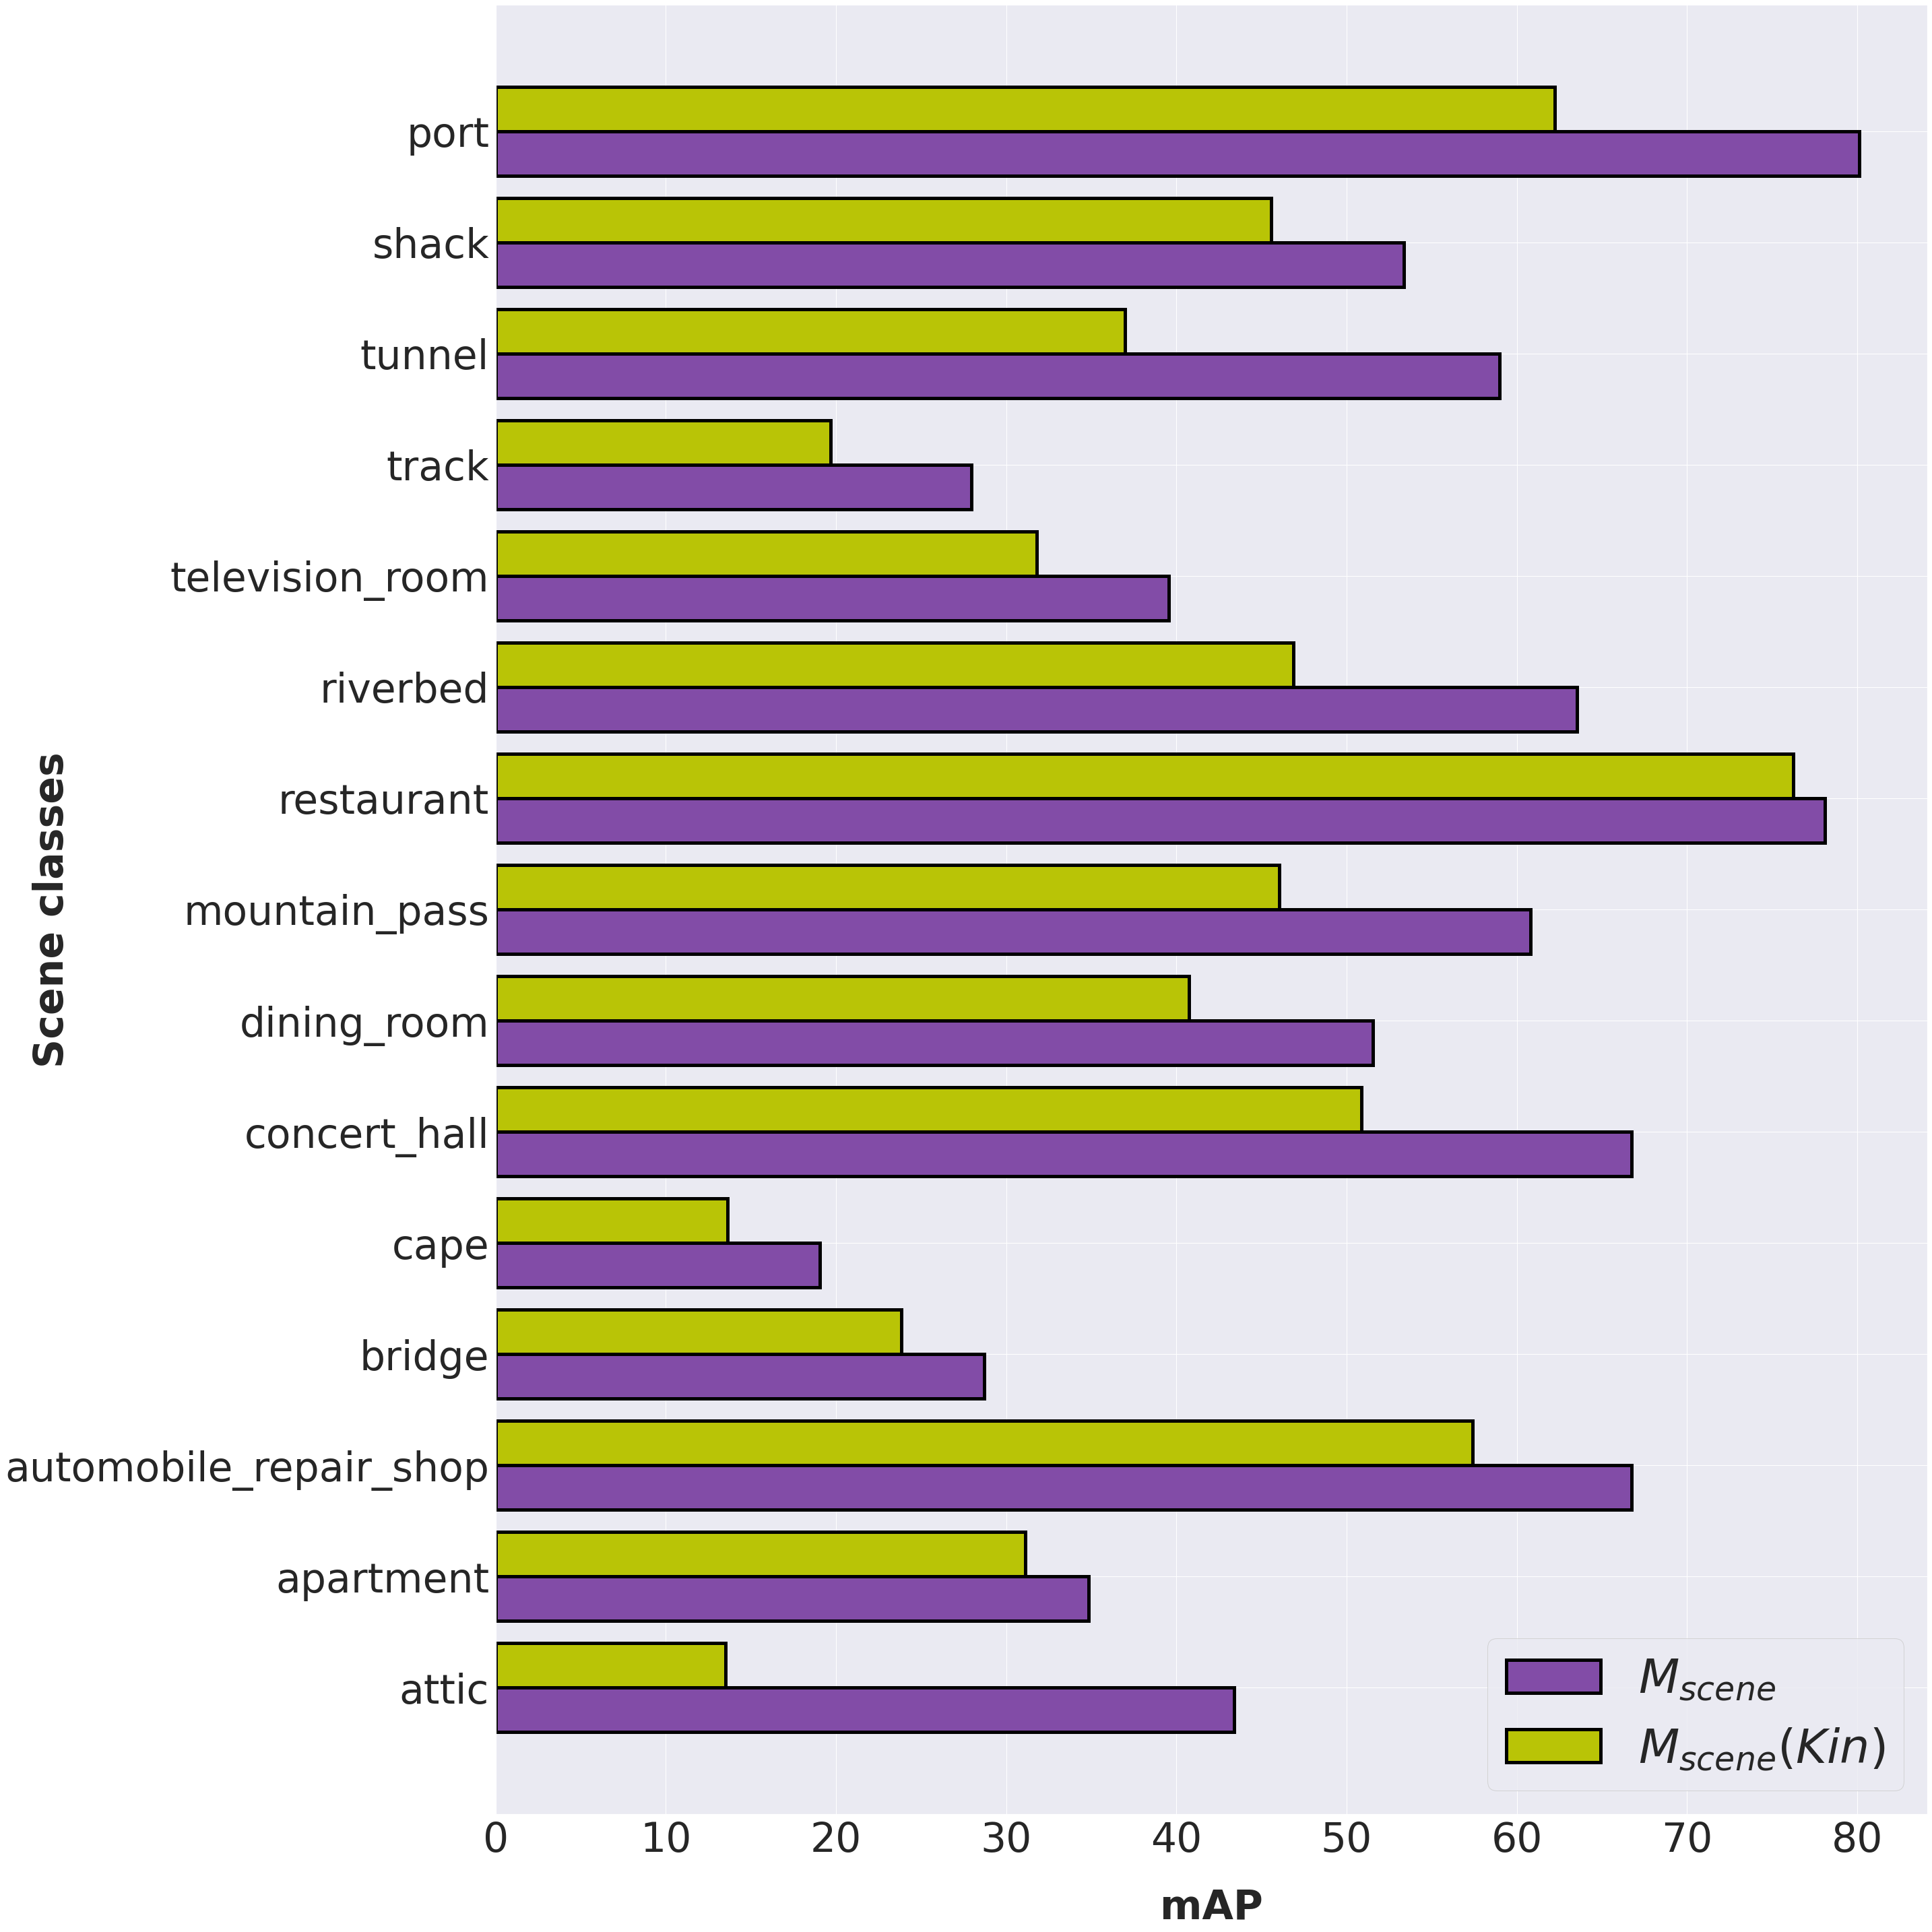
\includegraphics[width=0.6\textwidth]{figures/scene_gt_base_model_updated_legend.png}
    \caption{Sample scene classes in HVU where $M_{scene}$ performs better in comparison to $M_{scene}(Kin)$}. 
    \label{scenegtbase}
\end{figure}
\begin{table}[h!]
\centering
\resizebox{0.6\columnwidth}{!}{
\begin{tabular}{|cc|cc|}
\hline
\multicolumn{2}{|c|}{\textbf{HVU}}         & \multicolumn{2}{c|}{\textbf{Moviescope}}    \\ \hline
\multicolumn{1}{|c|}{\textbf{Model}}    & \textbf{mAP} & \multicolumn{1}{c|}{\textbf{Model}}      & \textbf{mAP} \\ \hline
\multicolumn{1}{|c|}{$M_{scene}$} &   55.92  & \multicolumn{1}{c|}{$M_{trailer}$} &  56.14   \\ \hline
\multicolumn{1}{|c|}{$M_{scene}(Kin)$}  &  56.05   & \multicolumn{1}{c|}{$M_{trailer}(Kin)$}  & 53.29    \\ \hline
\multicolumn{1}{|c|}{Late Fusion}             &  57.73   & \multicolumn{1}{c|}{Late Fusion}            &   56.29   \\ \hline
\end{tabular}
}
\vspace{3mm}
\caption{Impact of MovieCLIP pretrained features vs Kinetics pretrained features for $M_{scene}$ (HVU) and $M_{trailer}$ (Moviescope). Results reported are mean average precision (\textbf{mAP}) values. $Model(Kin)$: Model with Kinetics400 pretrained features, where $Model \in \{M_{scene},M_{trailer}\}$ }
\label{pretrain table}.
\end{table}
We consider the impact of MovieCLIP-based pretraining by fixing the fully connected architectures $M_{scene}$, $M_{trailer}$ and varying the input features. In the without MovieCLIP ($Kin$) pretraining setting, we extract 1024 dim features from Swin-B model pretrained on Kinetics400 for HVU and Moviescope datasets. 
From Table \ref{pretrain table}, we can see that the performance of $M_{scene}$ with MovieCLIP pretrained features is comparable to $M_{scene}(Kin)$, even when the domain of Kinetics400 \cite{kinetics400} is matched to HVU. Further, late fusion of prediction logits of $M_{scene}$ and  $M_{scene}(Kin)$ with equal weights improves the mAP to 57.73 for HVU, thus indicating the capture of complementary information when trained with movie data.
We show some class-wise analysis in Fig \ref{scenegtbase} to showcase the classes where MovieCLIP pretrained features improve upon Kinetics400 pretrained features. From Fig \ref{scenegtbase}, we can see that for certain classes present in our taxonomy like \textit{tunnel}, \textit{restaurant}, \textit{apartment}, \textit{attic} and \textit{concert hall}, $M_{scene}$ performs better when compared to $M_{scene}(Kin)$. Similar trends can be seen for HVU scene classes that are part of broader scene classes in our taxonomy like \textit{riverbed} (part of \textit{river}), \textit{mountain pass} (part of \textit{mountain}) and \textit{track} (part of \textit{race track}).
In case of Moviescope, $M_{trailer}$ 
results in improved performance (\textbf{56.14}) as compared to $M_{trailer}(Kin)$ (\textbf{53.29}), due to domain similarity with MovieCLIP dataset. 
\section{Ethical implications}
Visual scene recognition capabilities can help in uncovering biases associated with the portrayal of under-represented and marginalized characters in various settings. For example, women are portrayed more in indoor scenes like \textit{kitchen}, \textit{living room}, \textit{hospital} as compared to scenes like factory, laboratory, or battlefield. Further, characters from marginalized demographic groups are often depicted in the background w.r.t common visual scenes, thus having considerably less share of speaking time. Apart from the portrayal of characters, the usage of large-scale pretrained models like CLIP \cite{CLIP} can help diagnose the inherent biases associated with its predictions since it is trained on free-form data curated from the web. The proposed scheme of utilizing CLIP for weakly tagging datasets can reduce the costs associated with large-scale human expert-driven annotation processes.
\section{Takeaways}
From the visual scene context recognition in media content guided by multimodal signal, we have the following major takeaways:
\begin{itemize}
    \item \textbf{Role of pretrained knowledge:} Visual scene context signal can be extracted from media content through pretrained multimodal knowledge.
    \item \textbf{Domain-specific sources:} Domain-specific linguistic sources like screenplays provide rich sources of information for taxonomy curation.
    \item \textbf{Context-change tracking:} Shot-specific labels can enable tracking of visual scene context changes in dynamic content like movie videos.
    \item \textbf{Macro-level content understanding:} Pretrained visual scene representations can enable macro-level multimodal content understanding ( i.e. genre classification).
\end{itemize}
\section {Future work}
 Future directions include modeling of temporal transitions of visual scenes across shots, multimodal association between audio events and visual scenes, and multi-task modeling of visual scenes and related attributes like actions, time of day, and settings (interior and exterior).






